\chapter{Ultrafast Electron Diffractive Imaging}\label{chapter:diffraction}

One of the central motivations for the development of \gls{caeis} is their potential use as an electron source for the creation of molecular movies~\cite{van_der_geer_ultracold_2009}.
One of the stepping stones towards molecular movies is achieving single-shot ultrafast diffractive imaging and single-shot electron diffraction from gold nanofoils has already been demonstrated~\cite{speirs_single-shot_2015}.
If care is taken with the ionisation pathways the \gls{caes} is able to produce ultrafast bunches of cold electrons, as discussed in Section~\ref{section:two_stage_ionisation}~\cite{speirs_single-shot_2015,speirs_identification_2017,speirs_electron_2017}.
With improvements to the bunch current the next generation \gls{caes} will have the potential to do Bragg diffraction from simple samples that is both single-shot and ultrafast and eventually \gls{cdi}~\cite{mcculloch_cold_2016}.

Previous results from the \gls{caes} have shown diffraction from large crystalline samples using traditional crystallographic techniques~\cite{speirs_single-shot_2015,speirs_electron_2017}.
This chapter describes extensions to those results, namely demonstrating ultrafast diffraction from gold nanofoils and using a additional voltage bias applied to the sample holder to achieve the required beam energy for diffraction from polycrystalline aluminium.

\section{Crystallography}

Crystallography refers the the science of diffractive imaging from crystals and has been studied for over \unit[100]{years}, being the subject of the 1915 Nobel prize in physics~\cite{bragg_structure_1913}.
Crystallography has been an highly productive science generating numerous Nobel prizes and producing results such as the structure of DNA~\cite{franklin_structure_1953,dennis_eternal_2003}.
There are over 100,000 entries in the Protein Data Bank from from X-ray crystallography~\cite{noauthor_pdb_nodate}.
Crystallographic techniques have been under constant development and refinement since their inception.
The majority of crystallography to date has been performed using X-rays however relatively recent developments have utilised electrons as electron diffraction techniques are more versatile than those of X-rays~\cite{cowley_electron_1992}.

Due to the mature understanding of crystallographic techniques, crystallography is ideal for the first steps in demonstrating the capabilities of a \gls{caes}.
While the \gls{caes} is able to operate in \gls{cw} mode the performance with this apparatus has been optimised for pulse mode (see Section~\ref{section:pulse_vs_continuous}) and thus the results described in this chapter have been taken with pulsed bunches of electrons.

\subsection{Theory}

Crystalline structures consist of repeated sub-structures, unit cells, each with identical arrangements of atoms.
A perfect infinite crystal can be described as a lattice of unit cells where a set of basis vectors, $\mathbf{\hat{a}}$, $\mathbf{\hat{b}}$, and $\mathbf{\hat{c}}$, can be used to describe translations,
\begin{equation}
\mathbf{t} = u\mathbf{\hat{a}} + v\mathbf{\hat{b}} + w\mathbf{\hat{c}},
\end{equation}
where the integer coordinates $u$, $v$ and $w$ describe translation by a number of unit cells along each basis vector from some origin.
A primitive unit cell may contain one or more atoms and symmetry is sometimes more apparent if the unit cell consists of multiple primitive unit cells.

When a wave interacting with the crystal lattice interacts with a specific atom in every unit cell then the reflected waves will be in phase which creates a maxima in the diffraction pattern.
These planes in the crystal that these atoms line up on can be described by points in the reciprocal lattice.
The reciprocal lattice is described by the reciprocal lattice basis vectors, $\mathbf{\hat{a}^*}$, $\mathbf{\hat{b}^*}$, and $\mathbf{\hat{c}^*}$, where
\begin{align}
\mathbf{\hat{a}^*}&=\frac{2\pi\:\mathbf{\hat{b}}\times\mathbf{\hat{c}}}{\mathbf{\hat{a}}\cdot (\mathbf{\hat{b}} \times \mathbf{\hat{c}})},  &  \mathbf{\hat{b}^*}&=\frac{2\pi\:\mathbf{\hat{c}}\times\mathbf{\hat{a}}}{\mathbf{\hat{a}}\cdot (\mathbf{\hat{b}} \times \mathbf{\hat{c}})},  &  \mathbf{\hat{c}^*}&=\frac{2\pi\:\mathbf{\hat{a}}\times\mathbf{\hat{b}}}{\mathbf{\hat{a}}\cdot (\mathbf{\hat{b}} \times \mathbf{\hat{c}})}.
\end{align}
The $2\pi$ originates from the convention chosen for the wave-vector, $|\mathbf{k}|=2\pi/\lambda$. The reciprocal lattice vector is thus,
\begin{equation}
\mathbf{g} = h\mathbf{\hat{a}^*} + k\mathbf{\hat{b}^*} + l\mathbf{\hat{c}^*},
\end{equation}
where the integers $h$, $k$, and $l$ are known as the Miller indices.

Scattering events can be described by, $\mathbf{q}$, the scattering vector, which is the difference between the initial and final wavevectors, $\mathbf{k_0}$ and $\mathbf{k}$;
\begin{equation}
\mathbf{q} = \mathbf{k} - \mathbf{k_0}.
\end{equation}
In the case of elastically scatter waves, $|\mathbf{k}| = |\mathbf{k_0}|$.
Constructive interference occurs only where $\mathbf{q}$ is equal to a reciprocal lattice vector, so the scattering condition for crystals is
\begin{equation}
\mathbf{q} = \mathbf{g}.
\end{equation}
The relationship between the scattering vector and the scattering angle is
\begin{equation}\label{equation:diffraction_angle}
\left|\mathbf{q}\right| = 2\left|\mathbf{k_0}\right|\sin(\theta)
\end{equation}
where $\theta$ is the half angle between the initial and final wavevectors.
Due to the wavevector convention used the relation between real and reciprocal space distances is
\begin{equation}\label{equation:diffraction_distance}
\left|\mathbf{g}\right| = \frac{2\pi}{d_{hkl}},
\end{equation}
where $d_{hkl}$ is the distance between the set of planes described by the subscripted Miller indices.

If we combine Equations~\ref{equation:diffraction_angle} and \ref{equation:diffraction_distance} then we get the Bragg condition,
\begin{equation}
2d_{hkl}\sin\theta = n\lambda,
\end{equation}
where $n$ is the diffraction order.

The relative intensity of a wave with scattering vector $\mathbf{q}$ is given by
\begin{equation}
I(\mathbf{q}) = \left|\tilde{V}(\mathbf{q})\right|^2,
\end{equation}
where $\tilde{V}(\mathbf{q})$ is the Fourier transform of the crystal potential evaluated at $\mathbf{q}$ and we approximate to single-scattering events only.

The Fourier transform of the crystal potential, for an infinite crystal, can be written in terms of the structure factors, $V_g$,
\begin{equation}
\tilde{V}_{inf}(\mathbf{q}) = (2\pi)^3 \sum_g V_g \, \delta(\mathbf{q} - \mathbf{g}),
\end{equation}
where the sum takes the scattering contribution from all the reciprocal lattice points in to account, and the scattering condition is implemented with the Dirac delta.
The crystal basis affects the calculation of the structure factors for each reciprocal lattice point.
For a particular reciprocal lattice point, the structure factor is calculated by taking the position $\mathbf{x_j}$ and scattering factors $\tilde{V}_j$ for each atom, $j$, in the crystal basis:
\begin{equation}
V_g = \frac{1}{V_{cell}}\sum\tilde{V}_j(\mathbf{g})e^{-i\mathbf{g}\cdot\mathbf{x_j}}.
\end{equation}
$V_{cell}$ is the volume of the unit cell. The Fourier transform of an isolated atomic potential gives the scattering factors, $\tilde{V}_j(\mathbf{k})$ which are not the same as the Fourier transform of the whole crystal potential, $\tilde{V}(\mathbf{k})$.
$\tilde{V}_j(\mathbf{g})$ represents the probability that the atom $j$ will scatter an electron in to a direction corresponding to $\mathbf{g}$.
Scattering factors for most elements for a range of scattering angles and electron energies have been tabulated~\cite{peng_electron_1999}.
The numerical values for scattering factors are different for electrons and X-rays and are more commonly referred to as \emph{atomic form factors} in X-ray diffraction.

Due to the relatively low electron energy and bunch count used with the \gls{caes} it was necessary to use fairly thin samples to avoid overly attenuating the beam.
The use of thin samples causes a significant deviation from the infinite crystal assumption presented above.
For a finite crystal the potential can be calculated by incorporating the \emph{shape function}, $S(\mathbf{x})$, into the calculation;
\begin{equation}
V(\mathbf{x}) = V_{inf}(\mathbf{x})S(\mathbf{x})
\end{equation}
where
\begin{equation}
S(\mathbf{x}) = \left\{\begin{array}{l l}
1, & \text{for $\mathbf{x}$ inside the crystal} \\
0, & \text{otherwise}
\end{array}
\right.
\end{equation}

The Fourier transform of this potential, with the delta functions softened into sinc functions, is
\begin{equation}\label{equation:foil_ft_potential}
\tilde{V}(\mathbf{q}) = \sum_g V_g \: t_x  t_y  t_z \: \text{sinc}{\left( \frac{(q_x-g_x)t_x}{2} \right)} \,\, \text{sinc}{\left( \frac{(q_y-g_y)t_y}{2} \right)} \,\, \text{sinc}{\left( \frac{(q_z-g_z)t_z}{2} \right)}.
\end{equation}
Here, $t_x$, $t_y$ and $t_z$ are the sizes of the illuminated portions of the crystal.
As we use crystal foils in the experiments presented here , the sinc terms end up limiting towards delta functions in the two large dimensions, $x$ and $y$.
Equation~\ref{equation:foil_ft_potential} indicates that the diffraction condition does not need to be exactly met in order to diffract electrons in a particular direction.
The intensity of the diffracted spot will be reduced the further from meeting the diffraction condition the situation is.

\subsection{Diffraction Geometry}

A typical transmission electron diffraction apparatus uses a collimated beam of electrons, directed through the sample and then observes the angle to which the electrons diffract.
The use of a collimated beam simplifies the treatment of the reciprocal space as any diffracted electrons interacting with a specific reciprocal lattice point will be scattered in the same direction.
This results in a series of beamlets which correspond to the reflections where each beamlet is also collimated and of the same size an the incident beam.
In order to resolve the beamlets, they can either be propagated to the far field or passed through a lens in order to place the detector in the focal plane.

Propagating the beam to the far field requires satisfying the Fraunhofer condition,
\begin{equation}
W^2 \ll \Delta z\,\lambda,
\end{equation}
where $W$ is the transverse size of the initial beam, $\Delta z$ is the propagation distance and $\lambda$ is the electron wavelength.
The Fraunhofer condition requires either the beam size to be very small or the propagation distance to be very large.
The more practical method is to use a lens to artificially propagate the beam.
Lenses are the usual method used in \gls{tem} and the lenses are often combined with other sophisticated beam optics allowing for diffraction and imaging of a variety of samples and geometries.
The downside is the obvious complexity and cost associated with sophisticated beam optics.

A \gls{tem} consist of a relatively simple electron source combined with complex optics and in contrast our \gls{caes} consists of a complex electron source with relatively primitive beam optics.
For the measurements described in this chapter we only use a simple condenser lens between the source and sample to focus the beam on to the detector (the quadrupole lens discussed in Section~\ref{section:quadrupole} was added after these measurements were taken).
The beam was focused onto the detector in order to increase the intensity of the Bragg spots to inprove the \gls{snr}.
Due to the non-collimated beam there is a spread of incident angles at the crystalline samples that results in the reflected beamlets possessing the same convergence angle as the incident beam.
A schematic of the experimental setup is shown in Figure~\ref{figure:diffraction_geometry}.

\begin{figure}
    \center
    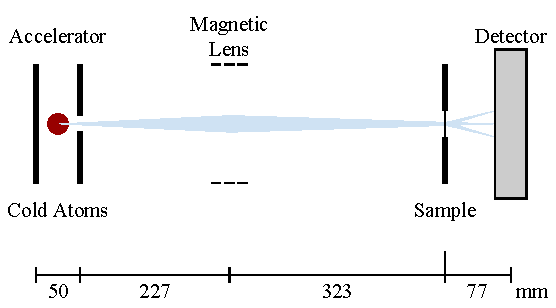
\includegraphics{part2/Figs/DiffractionGeometry.pdf}
    \caption[A schematic of the apparatus used for diffraction experiments.]{A schematic of the apparatus used in the diffraction experiments. The blue area indicates the path of the electrons.}
    \label{figure:diffraction_geometry}
\end{figure}

\section{Experimental Setup}

For the results presented in this chapter the apparatus described in Chapter~\ref{chapter:setup} was used to produce pulsed bunches of electrons.
The energy of the beam was close to the maximum the accelerator is able to produce, with the electrons given \unit[11.7]{keV}.

The majority of the data presented here was generated using electron bunches produced with ionisation pathways designed to maximise beam current.
The exception was the ultrafast diffraction measurements which used the ionisation pathways that produced ultrafast electron bunches, as described in Section~\ref{section:two_stage_ionisation}~\cite{speirs_single-shot_2015,speirs_identification_2017,speirs_electron_2017}.

These measurement did not take advantage of the beam shaping potential of the source instead the red excitation laser was given enough optical power to saturate the atom cloud, thus producing a higher beam current than is possible with shaping.
The excitation laser beam profile was Gaussian in beamshape with a \gls{fwhm} of \unit[80]{$\muup$m} at the \gls{mot} however, due to the laser intensity saturating the atom cloud, the electron bunches took on the shape of the atomic cloud which was roughly Gaussian.
The transverse bunch profile was not of particular concern as it was focused to a point at the detector.
The electron bunches at the source under similar conditions have been determined to have a Gaussian shape with a \gls{fwhm} of \unit[1.4]{mm} with a divergence of $\sigma_{\theta_x}$=\,\unit[0.3]{$\muup$rad} and thus a source emittance of $\epsilon_x$=\,\unit[50]{nm\,rad}~\cite{mcculloch_high-coherence_2013}.

The number of electrons per pulse when producing ns-duration bunches with this setup was measured with a Faraday cup to be $5\times10^5$ which corresponds to a bunch charge of \unit[80]{fC}.

The solenoid lens located just after the \gls{mot}, well before the samples, was used to focus the electron beam onto the detector with as small a convergence angle as practical.
These measurement were taken before the investigations into beam astigmatism discussed in Section~\ref{section:quadrupole} so there is some asymmetry apparent in the data.

\subsection{Sample Bias}\label{section:sample_bias}

As is shown in Section~\ref{section:aluminium_diffraction}, the maximum electron energy that the accelerator electrodes are able to provide is not sufficient to observe diffraction with some of the test samples.
If higher voltages were applied to the electrodes then they would undergo electrical breakdown making it impossible to generate higher energy electrons using the normal accelerator stuctures.
In order to provide a greater range of available particle energies a high voltage feedthrough was attached to the aluminium sample paddle so that incoming electrons would undergo a change in energy, dependant on the polarity and strength of the voltage bias.
The sample voltage bias could be up to \unit[8.5]{kV} before the high voltage cable would begin to short allowing for the beam energy to be increased to approximately \unit[20.2]{keV}.

\section{Results}

Presented in this section are a number of results demonstrating the capabilities of the \gls{caes} with crystalline samples.
This work presents the capstone to the diffraction studies conducted with this iteration of the \gls{caes} demonstrating diffraction from a number of samples and single-shot ultrafast diffraction from gold~\cite{speirs_single-shot_2015}.

\subsection{Transmission Diffraction from Gold}

The most successful diffraction was observed with a thin foil sample of single crystal gold.
The sample was a standard \unit[3]{mm} \gls{tem} sample of \unit[11]{nm} thick monocrystalline gold on a carbon grid.
Example diffraction patterns from the gold sample are shown in Figure~\ref{figure:au_diffraction} which shows 100-shot registered-averages and single shot diffraction patterns generated with high-current nanosecond-duration bunches and 1000-shot registered-averaged diffraction using relatively low-current ultrafast bunches.

\begin{figure}
    \center
    %% Creator: Matplotlib, PGF backend
%%
%% To include the figure in your LaTeX document, write
%%   \input{<filename>.pgf}
%%
%% Make sure the required packages are loaded in your preamble
%%   \usepackage{pgf}
%%
%% Figures using additional raster images can only be included by \input if
%% they are in the same directory as the main LaTeX file. For loading figures
%% from other directories you can use the `import` package
%%   \usepackage{import}
%% and then include the figures with
%%   \import{<path to file>}{<filename>.pgf}
%%
%% Matplotlib used the following preamble
%%
\begingroup%
\makeatletter%
\begin{pgfpicture}%
\pgfpathrectangle{\pgfpointorigin}{\pgfqpoint{5.710000in}{4.568000in}}%
\pgfusepath{use as bounding box, clip}%
\begin{pgfscope}%
\pgfsetbuttcap%
\pgfsetmiterjoin%
\definecolor{currentfill}{rgb}{1.000000,1.000000,1.000000}%
\pgfsetfillcolor{currentfill}%
\pgfsetlinewidth{0.000000pt}%
\definecolor{currentstroke}{rgb}{1.000000,1.000000,1.000000}%
\pgfsetstrokecolor{currentstroke}%
\pgfsetdash{}{0pt}%
\pgfpathmoveto{\pgfqpoint{0.000000in}{0.000000in}}%
\pgfpathlineto{\pgfqpoint{5.710000in}{0.000000in}}%
\pgfpathlineto{\pgfqpoint{5.710000in}{4.568000in}}%
\pgfpathlineto{\pgfqpoint{0.000000in}{4.568000in}}%
\pgfpathclose%
\pgfusepath{fill}%
\end{pgfscope}%
\begin{pgfscope}%
\pgfsetbuttcap%
\pgfsetmiterjoin%
\definecolor{currentfill}{rgb}{1.000000,1.000000,1.000000}%
\pgfsetfillcolor{currentfill}%
\pgfsetlinewidth{0.000000pt}%
\definecolor{currentstroke}{rgb}{0.000000,0.000000,0.000000}%
\pgfsetstrokecolor{currentstroke}%
\pgfsetstrokeopacity{0.000000}%
\pgfsetdash{}{0pt}%
\pgfpathmoveto{\pgfqpoint{0.713750in}{2.476064in}}%
\pgfpathlineto{\pgfqpoint{2.322932in}{2.476064in}}%
\pgfpathlineto{\pgfqpoint{2.322932in}{4.085245in}}%
\pgfpathlineto{\pgfqpoint{0.713750in}{4.085245in}}%
\pgfpathclose%
\pgfusepath{fill}%
\end{pgfscope}%
\begin{pgfscope}%
\pgfpathrectangle{\pgfqpoint{0.713750in}{2.476064in}}{\pgfqpoint{1.609182in}{1.609182in}} %
\pgfusepath{clip}%
\pgftext[at=\pgfqpoint{0.713750in}{2.476064in},left,bottom]{\pgfimage[interpolate=true,width=1.620000in,height=1.620000in]{gold_diffractions-img0.png}}%
\end{pgfscope}%
\begin{pgfscope}%
\pgfpathrectangle{\pgfqpoint{0.713750in}{2.476064in}}{\pgfqpoint{1.609182in}{1.609182in}} %
\pgfusepath{clip}%
\pgfsetbuttcap%
\pgfsetmiterjoin%
\pgfsetlinewidth{0.501875pt}%
\definecolor{currentstroke}{rgb}{1.000000,1.000000,1.000000}%
\pgfsetstrokecolor{currentstroke}%
\pgfsetdash{}{0pt}%
\pgfpathmoveto{\pgfqpoint{1.521152in}{3.096453in}}%
\pgfpathcurveto{\pgfqpoint{1.592572in}{3.096453in}}{\pgfqpoint{1.661139in}{3.124855in}}{\pgfqpoint{1.711640in}{3.175356in}}%
\pgfpathcurveto{\pgfqpoint{1.762141in}{3.225857in}}{\pgfqpoint{1.790542in}{3.294424in}}{\pgfqpoint{1.790542in}{3.365843in}}%
\pgfpathcurveto{\pgfqpoint{1.790542in}{3.437262in}}{\pgfqpoint{1.762141in}{3.505829in}}{\pgfqpoint{1.711640in}{3.556330in}}%
\pgfpathcurveto{\pgfqpoint{1.661139in}{3.606831in}}{\pgfqpoint{1.592572in}{3.635233in}}{\pgfqpoint{1.521152in}{3.635233in}}%
\pgfusepath{stroke}%
\end{pgfscope}%
\begin{pgfscope}%
\pgfpathrectangle{\pgfqpoint{0.713750in}{2.476064in}}{\pgfqpoint{1.609182in}{1.609182in}} %
\pgfusepath{clip}%
\pgfsetbuttcap%
\pgfsetmiterjoin%
\pgfsetlinewidth{0.501875pt}%
\definecolor{currentstroke}{rgb}{1.000000,1.000000,1.000000}%
\pgfsetstrokecolor{currentstroke}%
\pgfsetdash{}{0pt}%
\pgfpathmoveto{\pgfqpoint{1.521152in}{2.984868in}}%
\pgfpathcurveto{\pgfqpoint{1.622154in}{2.984868in}}{\pgfqpoint{1.719123in}{3.025034in}}{\pgfqpoint{1.790542in}{3.096453in}}%
\pgfpathcurveto{\pgfqpoint{1.861961in}{3.167872in}}{\pgfqpoint{1.902127in}{3.264841in}}{\pgfqpoint{1.902127in}{3.365843in}}%
\pgfpathcurveto{\pgfqpoint{1.902127in}{3.466845in}}{\pgfqpoint{1.861961in}{3.563814in}}{\pgfqpoint{1.790542in}{3.635233in}}%
\pgfpathcurveto{\pgfqpoint{1.719123in}{3.706652in}}{\pgfqpoint{1.622154in}{3.746818in}}{\pgfqpoint{1.521152in}{3.746818in}}%
\pgfusepath{stroke}%
\end{pgfscope}%
\begin{pgfscope}%
\pgfpathrectangle{\pgfqpoint{0.713750in}{2.476064in}}{\pgfqpoint{1.609182in}{1.609182in}} %
\pgfusepath{clip}%
\pgfsetbuttcap%
\pgfsetmiterjoin%
\pgfsetlinewidth{0.501875pt}%
\definecolor{currentstroke}{rgb}{1.000000,1.000000,1.000000}%
\pgfsetstrokecolor{currentstroke}%
\pgfsetdash{}{0pt}%
\pgfpathmoveto{\pgfqpoint{1.521152in}{2.827063in}}%
\pgfpathcurveto{\pgfqpoint{1.663991in}{2.827063in}}{\pgfqpoint{1.801125in}{2.883866in}}{\pgfqpoint{1.902127in}{2.984868in}}%
\pgfpathcurveto{\pgfqpoint{2.003129in}{3.085870in}}{\pgfqpoint{2.059932in}{3.223004in}}{\pgfqpoint{2.059932in}{3.365843in}}%
\pgfpathcurveto{\pgfqpoint{2.059932in}{3.508681in}}{\pgfqpoint{2.003129in}{3.645816in}}{\pgfqpoint{1.902127in}{3.746818in}}%
\pgfpathcurveto{\pgfqpoint{1.801125in}{3.847820in}}{\pgfqpoint{1.663991in}{3.904623in}}{\pgfqpoint{1.521152in}{3.904623in}}%
\pgfusepath{stroke}%
\end{pgfscope}%
\begin{pgfscope}%
\pgfpathrectangle{\pgfqpoint{0.713750in}{2.476064in}}{\pgfqpoint{1.609182in}{1.609182in}} %
\pgfusepath{clip}%
\pgfsetbuttcap%
\pgfsetmiterjoin%
\pgfsetlinewidth{0.501875pt}%
\definecolor{currentstroke}{rgb}{1.000000,1.000000,1.000000}%
\pgfsetstrokecolor{currentstroke}%
\pgfsetdash{}{0pt}%
\pgfpathmoveto{\pgfqpoint{1.521152in}{2.763469in}}%
\pgfpathcurveto{\pgfqpoint{1.680851in}{2.763469in}}{\pgfqpoint{1.834171in}{2.826977in}}{\pgfqpoint{1.947095in}{2.939900in}}%
\pgfpathcurveto{\pgfqpoint{2.060019in}{3.052824in}}{\pgfqpoint{2.123526in}{3.206145in}}{\pgfqpoint{2.123526in}{3.365843in}}%
\pgfpathcurveto{\pgfqpoint{2.123526in}{3.525541in}}{\pgfqpoint{2.060019in}{3.678862in}}{\pgfqpoint{1.947095in}{3.791786in}}%
\pgfpathcurveto{\pgfqpoint{1.834171in}{3.904709in}}{\pgfqpoint{1.680851in}{3.968217in}}{\pgfqpoint{1.521152in}{3.968217in}}%
\pgfusepath{stroke}%
\end{pgfscope}%
\begin{pgfscope}%
\pgfpathrectangle{\pgfqpoint{0.713750in}{2.476064in}}{\pgfqpoint{1.609182in}{1.609182in}} %
\pgfusepath{clip}%
\pgfsetbuttcap%
\pgfsetmiterjoin%
\pgfsetlinewidth{0.501875pt}%
\definecolor{currentstroke}{rgb}{1.000000,1.000000,1.000000}%
\pgfsetstrokecolor{currentstroke}%
\pgfsetdash{}{0pt}%
\pgfpathmoveto{\pgfqpoint{1.521152in}{2.603893in}}%
\pgfpathcurveto{\pgfqpoint{1.723157in}{2.603893in}}{\pgfqpoint{1.917094in}{2.684225in}}{\pgfqpoint{2.059932in}{2.827063in}}%
\pgfpathcurveto{\pgfqpoint{2.202771in}{2.969902in}}{\pgfqpoint{2.283102in}{3.163839in}}{\pgfqpoint{2.283102in}{3.365843in}}%
\pgfpathcurveto{\pgfqpoint{2.283102in}{3.567847in}}{\pgfqpoint{2.202771in}{3.761784in}}{\pgfqpoint{2.059932in}{3.904623in}}%
\pgfpathcurveto{\pgfqpoint{1.917094in}{4.047461in}}{\pgfqpoint{1.723157in}{4.127792in}}{\pgfqpoint{1.521152in}{4.127792in}}%
\pgfusepath{stroke}%
\end{pgfscope}%
\begin{pgfscope}%
\pgfpathrectangle{\pgfqpoint{0.713750in}{2.476064in}}{\pgfqpoint{1.609182in}{1.609182in}} %
\pgfusepath{clip}%
\pgfsetbuttcap%
\pgfsetmiterjoin%
\pgfsetlinewidth{0.501875pt}%
\definecolor{currentstroke}{rgb}{1.000000,1.000000,1.000000}%
\pgfsetstrokecolor{currentstroke}%
\pgfsetdash{}{0pt}%
\pgfpathmoveto{\pgfqpoint{1.521152in}{2.557673in}}%
\pgfpathcurveto{\pgfqpoint{1.735410in}{2.557673in}}{\pgfqpoint{1.941112in}{2.642878in}}{\pgfqpoint{2.092615in}{2.794381in}}%
\pgfpathcurveto{\pgfqpoint{2.244118in}{2.945884in}}{\pgfqpoint{2.329322in}{3.151585in}}{\pgfqpoint{2.329322in}{3.365843in}}%
\pgfpathcurveto{\pgfqpoint{2.329322in}{3.580101in}}{\pgfqpoint{2.244118in}{3.785802in}}{\pgfqpoint{2.092615in}{3.937305in}}%
\pgfpathcurveto{\pgfqpoint{1.941112in}{4.088808in}}{\pgfqpoint{1.735410in}{4.174012in}}{\pgfqpoint{1.521152in}{4.174012in}}%
\pgfusepath{stroke}%
\end{pgfscope}%
\begin{pgfscope}%
\pgfpathrectangle{\pgfqpoint{0.713750in}{2.476064in}}{\pgfqpoint{1.609182in}{1.609182in}} %
\pgfusepath{clip}%
\pgfsetbuttcap%
\pgfsetmiterjoin%
\pgfsetlinewidth{0.501875pt}%
\definecolor{currentstroke}{rgb}{1.000000,1.000000,1.000000}%
\pgfsetstrokecolor{currentstroke}%
\pgfsetdash{}{0pt}%
\pgfpathmoveto{\pgfqpoint{1.521152in}{2.513958in}}%
\pgfpathcurveto{\pgfqpoint{1.747000in}{2.513958in}}{\pgfqpoint{1.963828in}{2.603771in}}{\pgfqpoint{2.123526in}{2.763469in}}%
\pgfpathcurveto{\pgfqpoint{2.283225in}{2.923167in}}{\pgfqpoint{2.373038in}{3.139996in}}{\pgfqpoint{2.373038in}{3.365843in}}%
\pgfpathcurveto{\pgfqpoint{2.373038in}{3.591690in}}{\pgfqpoint{2.283225in}{3.808519in}}{\pgfqpoint{2.123526in}{3.968217in}}%
\pgfpathcurveto{\pgfqpoint{1.963828in}{4.127915in}}{\pgfqpoint{1.747000in}{4.217728in}}{\pgfqpoint{1.521152in}{4.217728in}}%
\pgfusepath{stroke}%
\end{pgfscope}%
\begin{pgfscope}%
\pgfpathrectangle{\pgfqpoint{0.713750in}{2.476064in}}{\pgfqpoint{1.609182in}{1.609182in}} %
\pgfusepath{clip}%
\pgfsetrectcap%
\pgfsetroundjoin%
\pgfsetlinewidth{0.501875pt}%
\definecolor{currentstroke}{rgb}{1.000000,1.000000,1.000000}%
\pgfsetstrokecolor{currentstroke}%
\pgfsetdash{}{0pt}%
\pgfpathmoveto{\pgfqpoint{0.818754in}{2.581067in}}%
\pgfpathlineto{\pgfqpoint{1.037415in}{2.581067in}}%
\pgfusepath{stroke}%
\end{pgfscope}%
\begin{pgfscope}%
\pgfpathrectangle{\pgfqpoint{0.713750in}{2.476064in}}{\pgfqpoint{1.609182in}{1.609182in}} %
\pgfusepath{clip}%
\pgfsetrectcap%
\pgfsetroundjoin%
\pgfsetlinewidth{0.501875pt}%
\definecolor{currentstroke}{rgb}{1.000000,1.000000,1.000000}%
\pgfsetstrokecolor{currentstroke}%
\pgfsetdash{}{0pt}%
\pgfpathmoveto{\pgfqpoint{0.818754in}{2.633569in}}%
\pgfpathlineto{\pgfqpoint{0.818754in}{2.528565in}}%
\pgfusepath{stroke}%
\end{pgfscope}%
\begin{pgfscope}%
\pgfpathrectangle{\pgfqpoint{0.713750in}{2.476064in}}{\pgfqpoint{1.609182in}{1.609182in}} %
\pgfusepath{clip}%
\pgfsetrectcap%
\pgfsetroundjoin%
\pgfsetlinewidth{0.501875pt}%
\definecolor{currentstroke}{rgb}{1.000000,1.000000,1.000000}%
\pgfsetstrokecolor{currentstroke}%
\pgfsetdash{}{0pt}%
\pgfpathmoveto{\pgfqpoint{1.037415in}{2.633569in}}%
\pgfpathlineto{\pgfqpoint{1.037415in}{2.528565in}}%
\pgfusepath{stroke}%
\end{pgfscope}%
\begin{pgfscope}%
\pgfsetrectcap%
\pgfsetmiterjoin%
\pgfsetlinewidth{1.003750pt}%
\definecolor{currentstroke}{rgb}{0.000000,0.000000,0.000000}%
\pgfsetstrokecolor{currentstroke}%
\pgfsetdash{}{0pt}%
\pgfpathmoveto{\pgfqpoint{0.713750in}{2.476064in}}%
\pgfpathlineto{\pgfqpoint{0.713750in}{4.085245in}}%
\pgfusepath{stroke}%
\end{pgfscope}%
\begin{pgfscope}%
\pgfsetrectcap%
\pgfsetmiterjoin%
\pgfsetlinewidth{1.003750pt}%
\definecolor{currentstroke}{rgb}{0.000000,0.000000,0.000000}%
\pgfsetstrokecolor{currentstroke}%
\pgfsetdash{}{0pt}%
\pgfpathmoveto{\pgfqpoint{0.713750in}{4.085245in}}%
\pgfpathlineto{\pgfqpoint{2.322932in}{4.085245in}}%
\pgfusepath{stroke}%
\end{pgfscope}%
\begin{pgfscope}%
\pgfsetrectcap%
\pgfsetmiterjoin%
\pgfsetlinewidth{1.003750pt}%
\definecolor{currentstroke}{rgb}{0.000000,0.000000,0.000000}%
\pgfsetstrokecolor{currentstroke}%
\pgfsetdash{}{0pt}%
\pgfpathmoveto{\pgfqpoint{0.713750in}{2.476064in}}%
\pgfpathlineto{\pgfqpoint{2.322932in}{2.476064in}}%
\pgfusepath{stroke}%
\end{pgfscope}%
\begin{pgfscope}%
\pgfsetrectcap%
\pgfsetmiterjoin%
\pgfsetlinewidth{1.003750pt}%
\definecolor{currentstroke}{rgb}{0.000000,0.000000,0.000000}%
\pgfsetstrokecolor{currentstroke}%
\pgfsetdash{}{0pt}%
\pgfpathmoveto{\pgfqpoint{2.322932in}{2.476064in}}%
\pgfpathlineto{\pgfqpoint{2.322932in}{4.085245in}}%
\pgfusepath{stroke}%
\end{pgfscope}%
\begin{pgfscope}%
\definecolor{textcolor}{rgb}{1.000000,1.000000,1.000000}%
\pgfsetstrokecolor{textcolor}%
\pgfsetfillcolor{textcolor}%
\pgftext[x=0.980586in,y=2.638819in,,bottom]{\color{textcolor}\fontsize{11.000000}{13.200000}\selectfont 5\,\AA\(\displaystyle ^{-1}\)}%
\end{pgfscope}%
\begin{pgfscope}%
\pgftext[x=1.518341in,y=4.154690in,,base]{\fontsize{12.000000}{14.400000}\selectfont (a)}%
\end{pgfscope}%
\begin{pgfscope}%
\pgfsetbuttcap%
\pgfsetmiterjoin%
\definecolor{currentfill}{rgb}{1.000000,1.000000,1.000000}%
\pgfsetfillcolor{currentfill}%
\pgfsetlinewidth{0.000000pt}%
\definecolor{currentstroke}{rgb}{0.000000,0.000000,0.000000}%
\pgfsetstrokecolor{currentstroke}%
\pgfsetstrokeopacity{0.000000}%
\pgfsetdash{}{0pt}%
\pgfpathmoveto{\pgfqpoint{0.713750in}{0.456800in}}%
\pgfpathlineto{\pgfqpoint{2.322932in}{0.456800in}}%
\pgfpathlineto{\pgfqpoint{2.322932in}{2.117891in}}%
\pgfpathlineto{\pgfqpoint{0.713750in}{2.117891in}}%
\pgfpathclose%
\pgfusepath{fill}%
\end{pgfscope}%
\begin{pgfscope}%
\pgfpathrectangle{\pgfqpoint{0.713750in}{0.456800in}}{\pgfqpoint{1.609182in}{1.661091in}} %
\pgfusepath{clip}%
\pgfsetrectcap%
\pgfsetroundjoin%
\pgfsetlinewidth{1.003750pt}%
\definecolor{currentstroke}{rgb}{0.600000,0.000000,0.000000}%
\pgfsetstrokecolor{currentstroke}%
\pgfsetdash{}{0pt}%
\pgfpathmoveto{\pgfqpoint{1.075752in}{0.456800in}}%
\pgfpathlineto{\pgfqpoint{1.075752in}{2.117891in}}%
\pgfusepath{stroke}%
\end{pgfscope}%
\begin{pgfscope}%
\pgfpathrectangle{\pgfqpoint{0.713750in}{0.456800in}}{\pgfqpoint{1.609182in}{1.661091in}} %
\pgfusepath{clip}%
\pgfsetrectcap%
\pgfsetroundjoin%
\pgfsetlinewidth{1.003750pt}%
\definecolor{currentstroke}{rgb}{0.600000,0.000000,0.000000}%
\pgfsetstrokecolor{currentstroke}%
\pgfsetdash{}{0pt}%
\pgfpathmoveto{\pgfqpoint{1.225698in}{0.456800in}}%
\pgfpathlineto{\pgfqpoint{1.225698in}{2.117891in}}%
\pgfusepath{stroke}%
\end{pgfscope}%
\begin{pgfscope}%
\pgfpathrectangle{\pgfqpoint{0.713750in}{0.456800in}}{\pgfqpoint{1.609182in}{1.661091in}} %
\pgfusepath{clip}%
\pgfsetrectcap%
\pgfsetroundjoin%
\pgfsetlinewidth{1.003750pt}%
\definecolor{currentstroke}{rgb}{0.600000,0.000000,0.000000}%
\pgfsetstrokecolor{currentstroke}%
\pgfsetdash{}{0pt}%
\pgfpathmoveto{\pgfqpoint{1.437754in}{0.456800in}}%
\pgfpathlineto{\pgfqpoint{1.437754in}{2.117891in}}%
\pgfusepath{stroke}%
\end{pgfscope}%
\begin{pgfscope}%
\pgfpathrectangle{\pgfqpoint{0.713750in}{0.456800in}}{\pgfqpoint{1.609182in}{1.661091in}} %
\pgfusepath{clip}%
\pgfsetrectcap%
\pgfsetroundjoin%
\pgfsetlinewidth{1.003750pt}%
\definecolor{currentstroke}{rgb}{0.600000,0.000000,0.000000}%
\pgfsetstrokecolor{currentstroke}%
\pgfsetdash{}{0pt}%
\pgfpathmoveto{\pgfqpoint{1.523211in}{0.456800in}}%
\pgfpathlineto{\pgfqpoint{1.523211in}{2.117891in}}%
\pgfusepath{stroke}%
\end{pgfscope}%
\begin{pgfscope}%
\pgfpathrectangle{\pgfqpoint{0.713750in}{0.456800in}}{\pgfqpoint{1.609182in}{1.661091in}} %
\pgfusepath{clip}%
\pgfsetrectcap%
\pgfsetroundjoin%
\pgfsetlinewidth{1.003750pt}%
\definecolor{currentstroke}{rgb}{0.600000,0.000000,0.000000}%
\pgfsetstrokecolor{currentstroke}%
\pgfsetdash{}{0pt}%
\pgfpathmoveto{\pgfqpoint{1.737646in}{0.456800in}}%
\pgfpathlineto{\pgfqpoint{1.737646in}{2.117891in}}%
\pgfusepath{stroke}%
\end{pgfscope}%
\begin{pgfscope}%
\pgfpathrectangle{\pgfqpoint{0.713750in}{0.456800in}}{\pgfqpoint{1.609182in}{1.661091in}} %
\pgfusepath{clip}%
\pgfsetrectcap%
\pgfsetroundjoin%
\pgfsetlinewidth{1.003750pt}%
\definecolor{currentstroke}{rgb}{0.600000,0.000000,0.000000}%
\pgfsetstrokecolor{currentstroke}%
\pgfsetdash{}{0pt}%
\pgfpathmoveto{\pgfqpoint{1.799755in}{0.456800in}}%
\pgfpathlineto{\pgfqpoint{1.799755in}{2.117891in}}%
\pgfusepath{stroke}%
\end{pgfscope}%
\begin{pgfscope}%
\pgfpathrectangle{\pgfqpoint{0.713750in}{0.456800in}}{\pgfqpoint{1.609182in}{1.661091in}} %
\pgfusepath{clip}%
\pgfsetrectcap%
\pgfsetroundjoin%
\pgfsetlinewidth{1.003750pt}%
\definecolor{currentstroke}{rgb}{0.600000,0.000000,0.000000}%
\pgfsetstrokecolor{currentstroke}%
\pgfsetdash{}{0pt}%
\pgfpathmoveto{\pgfqpoint{1.858500in}{0.456800in}}%
\pgfpathlineto{\pgfqpoint{1.858500in}{2.117891in}}%
\pgfusepath{stroke}%
\end{pgfscope}%
\begin{pgfscope}%
\pgfpathrectangle{\pgfqpoint{0.713750in}{0.456800in}}{\pgfqpoint{1.609182in}{1.661091in}} %
\pgfusepath{clip}%
\pgfsetrectcap%
\pgfsetroundjoin%
\pgfsetlinewidth{1.003750pt}%
\definecolor{currentstroke}{rgb}{0.309804,0.478431,0.682353}%
\pgfsetstrokecolor{currentstroke}%
\pgfsetdash{}{0pt}%
\pgfpathmoveto{\pgfqpoint{0.715273in}{1.789294in}}%
\pgfpathlineto{\pgfqpoint{0.758287in}{1.788901in}}%
\pgfpathlineto{\pgfqpoint{0.763664in}{1.787252in}}%
\pgfpathlineto{\pgfqpoint{0.769041in}{1.780961in}}%
\pgfpathlineto{\pgfqpoint{0.774417in}{1.767982in}}%
\pgfpathlineto{\pgfqpoint{0.785171in}{1.725905in}}%
\pgfpathlineto{\pgfqpoint{0.795925in}{1.676883in}}%
\pgfpathlineto{\pgfqpoint{0.801301in}{1.649870in}}%
\pgfpathlineto{\pgfqpoint{0.833562in}{1.528784in}}%
\pgfpathlineto{\pgfqpoint{0.844316in}{1.498371in}}%
\pgfpathlineto{\pgfqpoint{0.855069in}{1.473168in}}%
\pgfpathlineto{\pgfqpoint{0.898084in}{1.400408in}}%
\pgfpathlineto{\pgfqpoint{0.903460in}{1.395300in}}%
\pgfpathlineto{\pgfqpoint{0.908837in}{1.384119in}}%
\pgfpathlineto{\pgfqpoint{0.914214in}{1.376619in}}%
\pgfpathlineto{\pgfqpoint{0.919591in}{1.364603in}}%
\pgfpathlineto{\pgfqpoint{0.930344in}{1.349341in}}%
\pgfpathlineto{\pgfqpoint{0.946475in}{1.324316in}}%
\pgfpathlineto{\pgfqpoint{0.957228in}{1.311259in}}%
\pgfpathlineto{\pgfqpoint{0.962605in}{1.305751in}}%
\pgfpathlineto{\pgfqpoint{0.978735in}{1.295692in}}%
\pgfpathlineto{\pgfqpoint{0.984112in}{1.293747in}}%
\pgfpathlineto{\pgfqpoint{0.994866in}{1.294061in}}%
\pgfpathlineto{\pgfqpoint{1.000242in}{1.297448in}}%
\pgfpathlineto{\pgfqpoint{1.005619in}{1.298051in}}%
\pgfpathlineto{\pgfqpoint{1.010996in}{1.303393in}}%
\pgfpathlineto{\pgfqpoint{1.016373in}{1.306064in}}%
\pgfpathlineto{\pgfqpoint{1.021750in}{1.314967in}}%
\pgfpathlineto{\pgfqpoint{1.027126in}{1.317991in}}%
\pgfpathlineto{\pgfqpoint{1.032503in}{1.332438in}}%
\pgfpathlineto{\pgfqpoint{1.037880in}{1.333413in}}%
\pgfpathlineto{\pgfqpoint{1.043257in}{1.351432in}}%
\pgfpathlineto{\pgfqpoint{1.054010in}{1.368365in}}%
\pgfpathlineto{\pgfqpoint{1.070141in}{1.390521in}}%
\pgfpathlineto{\pgfqpoint{1.075518in}{1.391420in}}%
\pgfpathlineto{\pgfqpoint{1.080894in}{1.390512in}}%
\pgfpathlineto{\pgfqpoint{1.086271in}{1.381289in}}%
\pgfpathlineto{\pgfqpoint{1.091648in}{1.375504in}}%
\pgfpathlineto{\pgfqpoint{1.097025in}{1.358882in}}%
\pgfpathlineto{\pgfqpoint{1.102401in}{1.347692in}}%
\pgfpathlineto{\pgfqpoint{1.107778in}{1.325466in}}%
\pgfpathlineto{\pgfqpoint{1.113155in}{1.315115in}}%
\pgfpathlineto{\pgfqpoint{1.118532in}{1.291836in}}%
\pgfpathlineto{\pgfqpoint{1.123909in}{1.280342in}}%
\pgfpathlineto{\pgfqpoint{1.129285in}{1.257192in}}%
\pgfpathlineto{\pgfqpoint{1.134662in}{1.248095in}}%
\pgfpathlineto{\pgfqpoint{1.140039in}{1.229829in}}%
\pgfpathlineto{\pgfqpoint{1.145416in}{1.224264in}}%
\pgfpathlineto{\pgfqpoint{1.150793in}{1.212824in}}%
\pgfpathlineto{\pgfqpoint{1.166923in}{1.203735in}}%
\pgfpathlineto{\pgfqpoint{1.172300in}{1.201823in}}%
\pgfpathlineto{\pgfqpoint{1.177676in}{1.204093in}}%
\pgfpathlineto{\pgfqpoint{1.183053in}{1.207632in}}%
\pgfpathlineto{\pgfqpoint{1.188430in}{1.215670in}}%
\pgfpathlineto{\pgfqpoint{1.199184in}{1.235770in}}%
\pgfpathlineto{\pgfqpoint{1.204560in}{1.242029in}}%
\pgfpathlineto{\pgfqpoint{1.209937in}{1.250233in}}%
\pgfpathlineto{\pgfqpoint{1.220691in}{1.261251in}}%
\pgfpathlineto{\pgfqpoint{1.226068in}{1.269048in}}%
\pgfpathlineto{\pgfqpoint{1.231444in}{1.269626in}}%
\pgfpathlineto{\pgfqpoint{1.242198in}{1.249784in}}%
\pgfpathlineto{\pgfqpoint{1.258328in}{1.215121in}}%
\pgfpathlineto{\pgfqpoint{1.263705in}{1.205401in}}%
\pgfpathlineto{\pgfqpoint{1.274459in}{1.172955in}}%
\pgfpathlineto{\pgfqpoint{1.285212in}{1.151668in}}%
\pgfpathlineto{\pgfqpoint{1.295966in}{1.137801in}}%
\pgfpathlineto{\pgfqpoint{1.306719in}{1.125532in}}%
\pgfpathlineto{\pgfqpoint{1.312096in}{1.122215in}}%
\pgfpathlineto{\pgfqpoint{1.328226in}{1.104406in}}%
\pgfpathlineto{\pgfqpoint{1.333603in}{1.098782in}}%
\pgfpathlineto{\pgfqpoint{1.349734in}{1.077613in}}%
\pgfpathlineto{\pgfqpoint{1.360487in}{1.065808in}}%
\pgfpathlineto{\pgfqpoint{1.365864in}{1.062680in}}%
\pgfpathlineto{\pgfqpoint{1.371241in}{1.057997in}}%
\pgfpathlineto{\pgfqpoint{1.376618in}{1.055552in}}%
\pgfpathlineto{\pgfqpoint{1.387371in}{1.049120in}}%
\pgfpathlineto{\pgfqpoint{1.392748in}{1.046029in}}%
\pgfpathlineto{\pgfqpoint{1.403501in}{1.044080in}}%
\pgfpathlineto{\pgfqpoint{1.408878in}{1.043844in}}%
\pgfpathlineto{\pgfqpoint{1.435762in}{1.048693in}}%
\pgfpathlineto{\pgfqpoint{1.441139in}{1.051791in}}%
\pgfpathlineto{\pgfqpoint{1.451893in}{1.052155in}}%
\pgfpathlineto{\pgfqpoint{1.457269in}{1.049971in}}%
\pgfpathlineto{\pgfqpoint{1.462646in}{1.050460in}}%
\pgfpathlineto{\pgfqpoint{1.468023in}{1.048641in}}%
\pgfpathlineto{\pgfqpoint{1.473400in}{1.050522in}}%
\pgfpathlineto{\pgfqpoint{1.478776in}{1.049462in}}%
\pgfpathlineto{\pgfqpoint{1.484153in}{1.054232in}}%
\pgfpathlineto{\pgfqpoint{1.489530in}{1.055151in}}%
\pgfpathlineto{\pgfqpoint{1.494907in}{1.060846in}}%
\pgfpathlineto{\pgfqpoint{1.500284in}{1.064479in}}%
\pgfpathlineto{\pgfqpoint{1.505660in}{1.070730in}}%
\pgfpathlineto{\pgfqpoint{1.521791in}{1.081920in}}%
\pgfpathlineto{\pgfqpoint{1.532544in}{1.082161in}}%
\pgfpathlineto{\pgfqpoint{1.537921in}{1.079488in}}%
\pgfpathlineto{\pgfqpoint{1.548675in}{1.065502in}}%
\pgfpathlineto{\pgfqpoint{1.559428in}{1.045188in}}%
\pgfpathlineto{\pgfqpoint{1.586312in}{0.999045in}}%
\pgfpathlineto{\pgfqpoint{1.597066in}{0.984224in}}%
\pgfpathlineto{\pgfqpoint{1.602443in}{0.978739in}}%
\pgfpathlineto{\pgfqpoint{1.613196in}{0.973523in}}%
\pgfpathlineto{\pgfqpoint{1.623950in}{0.971524in}}%
\pgfpathlineto{\pgfqpoint{1.640080in}{0.970552in}}%
\pgfpathlineto{\pgfqpoint{1.661587in}{0.958409in}}%
\pgfpathlineto{\pgfqpoint{1.677718in}{0.947478in}}%
\pgfpathlineto{\pgfqpoint{1.688471in}{0.943732in}}%
\pgfpathlineto{\pgfqpoint{1.709978in}{0.936691in}}%
\pgfpathlineto{\pgfqpoint{1.731485in}{0.937472in}}%
\pgfpathlineto{\pgfqpoint{1.742239in}{0.940319in}}%
\pgfpathlineto{\pgfqpoint{1.747616in}{0.944197in}}%
\pgfpathlineto{\pgfqpoint{1.752993in}{0.945195in}}%
\pgfpathlineto{\pgfqpoint{1.763746in}{0.945407in}}%
\pgfpathlineto{\pgfqpoint{1.779876in}{0.948317in}}%
\pgfpathlineto{\pgfqpoint{1.806760in}{0.940724in}}%
\pgfpathlineto{\pgfqpoint{1.833644in}{0.925826in}}%
\pgfpathlineto{\pgfqpoint{1.839021in}{0.923382in}}%
\pgfpathlineto{\pgfqpoint{1.860528in}{0.907702in}}%
\pgfpathlineto{\pgfqpoint{1.865905in}{0.905769in}}%
\pgfpathlineto{\pgfqpoint{1.871282in}{0.901553in}}%
\pgfpathlineto{\pgfqpoint{1.876659in}{0.901004in}}%
\pgfpathlineto{\pgfqpoint{1.882035in}{0.897995in}}%
\pgfpathlineto{\pgfqpoint{1.887412in}{0.897515in}}%
\pgfpathlineto{\pgfqpoint{1.898166in}{0.894954in}}%
\pgfpathlineto{\pgfqpoint{1.903543in}{0.890623in}}%
\pgfpathlineto{\pgfqpoint{1.908919in}{0.888902in}}%
\pgfpathlineto{\pgfqpoint{1.914296in}{0.885755in}}%
\pgfpathlineto{\pgfqpoint{1.962687in}{0.876843in}}%
\pgfpathlineto{\pgfqpoint{1.973441in}{0.875431in}}%
\pgfpathlineto{\pgfqpoint{1.978818in}{0.874236in}}%
\pgfpathlineto{\pgfqpoint{1.989571in}{0.875694in}}%
\pgfpathlineto{\pgfqpoint{2.027209in}{0.884465in}}%
\pgfpathlineto{\pgfqpoint{2.037962in}{0.884940in}}%
\pgfpathlineto{\pgfqpoint{2.059469in}{0.886381in}}%
\pgfpathlineto{\pgfqpoint{2.064846in}{0.885276in}}%
\pgfpathlineto{\pgfqpoint{2.075600in}{0.879250in}}%
\pgfpathlineto{\pgfqpoint{2.086353in}{0.877931in}}%
\pgfpathlineto{\pgfqpoint{2.091730in}{0.880596in}}%
\pgfpathlineto{\pgfqpoint{2.097107in}{0.877577in}}%
\pgfpathlineto{\pgfqpoint{2.107860in}{0.874138in}}%
\pgfpathlineto{\pgfqpoint{2.113237in}{0.871475in}}%
\pgfpathlineto{\pgfqpoint{2.129368in}{0.869300in}}%
\pgfpathlineto{\pgfqpoint{2.140121in}{0.869023in}}%
\pgfpathlineto{\pgfqpoint{2.156251in}{0.857220in}}%
\pgfpathlineto{\pgfqpoint{2.161628in}{0.858470in}}%
\pgfpathlineto{\pgfqpoint{2.167005in}{0.863594in}}%
\pgfpathlineto{\pgfqpoint{2.172382in}{0.865431in}}%
\pgfpathlineto{\pgfqpoint{2.177759in}{0.864907in}}%
\pgfpathlineto{\pgfqpoint{2.183135in}{0.865655in}}%
\pgfpathlineto{\pgfqpoint{2.188512in}{0.862276in}}%
\pgfpathlineto{\pgfqpoint{2.199266in}{0.862634in}}%
\pgfpathlineto{\pgfqpoint{2.204643in}{0.864079in}}%
\pgfpathlineto{\pgfqpoint{2.210019in}{0.862755in}}%
\pgfpathlineto{\pgfqpoint{2.220773in}{0.865795in}}%
\pgfpathlineto{\pgfqpoint{2.231526in}{0.868510in}}%
\pgfpathlineto{\pgfqpoint{2.236903in}{0.873255in}}%
\pgfpathlineto{\pgfqpoint{2.242280in}{0.871803in}}%
\pgfpathlineto{\pgfqpoint{2.247657in}{0.873605in}}%
\pgfpathlineto{\pgfqpoint{2.253034in}{0.869279in}}%
\pgfpathlineto{\pgfqpoint{2.258410in}{0.870080in}}%
\pgfpathlineto{\pgfqpoint{2.263787in}{0.869042in}}%
\pgfpathlineto{\pgfqpoint{2.279918in}{0.875543in}}%
\pgfpathlineto{\pgfqpoint{2.285294in}{0.874949in}}%
\pgfpathlineto{\pgfqpoint{2.290671in}{0.869405in}}%
\pgfpathlineto{\pgfqpoint{2.296048in}{0.869008in}}%
\pgfpathlineto{\pgfqpoint{2.301425in}{0.873065in}}%
\pgfpathlineto{\pgfqpoint{2.306801in}{0.872596in}}%
\pgfpathlineto{\pgfqpoint{2.312178in}{0.873540in}}%
\pgfpathlineto{\pgfqpoint{2.317555in}{0.867078in}}%
\pgfpathlineto{\pgfqpoint{2.322932in}{0.870839in}}%
\pgfpathlineto{\pgfqpoint{2.322932in}{0.870839in}}%
\pgfusepath{stroke}%
\end{pgfscope}%
\begin{pgfscope}%
\pgfsetrectcap%
\pgfsetmiterjoin%
\pgfsetlinewidth{1.003750pt}%
\definecolor{currentstroke}{rgb}{0.000000,0.000000,0.000000}%
\pgfsetstrokecolor{currentstroke}%
\pgfsetdash{}{0pt}%
\pgfpathmoveto{\pgfqpoint{0.713750in}{0.456800in}}%
\pgfpathlineto{\pgfqpoint{0.713750in}{2.117891in}}%
\pgfusepath{stroke}%
\end{pgfscope}%
\begin{pgfscope}%
\pgfsetrectcap%
\pgfsetmiterjoin%
\pgfsetlinewidth{1.003750pt}%
\definecolor{currentstroke}{rgb}{0.000000,0.000000,0.000000}%
\pgfsetstrokecolor{currentstroke}%
\pgfsetdash{}{0pt}%
\pgfpathmoveto{\pgfqpoint{0.713750in}{2.117891in}}%
\pgfpathlineto{\pgfqpoint{2.322932in}{2.117891in}}%
\pgfusepath{stroke}%
\end{pgfscope}%
\begin{pgfscope}%
\pgfsetrectcap%
\pgfsetmiterjoin%
\pgfsetlinewidth{1.003750pt}%
\definecolor{currentstroke}{rgb}{0.000000,0.000000,0.000000}%
\pgfsetstrokecolor{currentstroke}%
\pgfsetdash{}{0pt}%
\pgfpathmoveto{\pgfqpoint{0.713750in}{0.456800in}}%
\pgfpathlineto{\pgfqpoint{2.322932in}{0.456800in}}%
\pgfusepath{stroke}%
\end{pgfscope}%
\begin{pgfscope}%
\pgfsetrectcap%
\pgfsetmiterjoin%
\pgfsetlinewidth{1.003750pt}%
\definecolor{currentstroke}{rgb}{0.000000,0.000000,0.000000}%
\pgfsetstrokecolor{currentstroke}%
\pgfsetdash{}{0pt}%
\pgfpathmoveto{\pgfqpoint{2.322932in}{0.456800in}}%
\pgfpathlineto{\pgfqpoint{2.322932in}{2.117891in}}%
\pgfusepath{stroke}%
\end{pgfscope}%
\begin{pgfscope}%
\pgfsetbuttcap%
\pgfsetroundjoin%
\definecolor{currentfill}{rgb}{0.000000,0.000000,0.000000}%
\pgfsetfillcolor{currentfill}%
\pgfsetlinewidth{0.501875pt}%
\definecolor{currentstroke}{rgb}{0.000000,0.000000,0.000000}%
\pgfsetstrokecolor{currentstroke}%
\pgfsetdash{}{0pt}%
\pgfsys@defobject{currentmarker}{\pgfqpoint{0.000000in}{0.000000in}}{\pgfqpoint{0.000000in}{0.055556in}}{%
\pgfpathmoveto{\pgfqpoint{0.000000in}{0.000000in}}%
\pgfpathlineto{\pgfqpoint{0.000000in}{0.055556in}}%
\pgfusepath{stroke,fill}%
}%
\begin{pgfscope}%
\pgfsys@transformshift{0.713750in}{0.456800in}%
\pgfsys@useobject{currentmarker}{}%
\end{pgfscope}%
\end{pgfscope}%
\begin{pgfscope}%
\pgfsetbuttcap%
\pgfsetroundjoin%
\definecolor{currentfill}{rgb}{0.000000,0.000000,0.000000}%
\pgfsetfillcolor{currentfill}%
\pgfsetlinewidth{0.501875pt}%
\definecolor{currentstroke}{rgb}{0.000000,0.000000,0.000000}%
\pgfsetstrokecolor{currentstroke}%
\pgfsetdash{}{0pt}%
\pgfsys@defobject{currentmarker}{\pgfqpoint{0.000000in}{-0.055556in}}{\pgfqpoint{0.000000in}{0.000000in}}{%
\pgfpathmoveto{\pgfqpoint{0.000000in}{0.000000in}}%
\pgfpathlineto{\pgfqpoint{0.000000in}{-0.055556in}}%
\pgfusepath{stroke,fill}%
}%
\begin{pgfscope}%
\pgfsys@transformshift{0.713750in}{2.117891in}%
\pgfsys@useobject{currentmarker}{}%
\end{pgfscope}%
\end{pgfscope}%
\begin{pgfscope}%
\pgftext[x=0.713750in,y=0.401244in,,top]{\fontsize{10.000000}{12.000000}\selectfont \(\displaystyle 0\)}%
\end{pgfscope}%
\begin{pgfscope}%
\pgfsetbuttcap%
\pgfsetroundjoin%
\definecolor{currentfill}{rgb}{0.000000,0.000000,0.000000}%
\pgfsetfillcolor{currentfill}%
\pgfsetlinewidth{0.501875pt}%
\definecolor{currentstroke}{rgb}{0.000000,0.000000,0.000000}%
\pgfsetstrokecolor{currentstroke}%
\pgfsetdash{}{0pt}%
\pgfsys@defobject{currentmarker}{\pgfqpoint{0.000000in}{0.000000in}}{\pgfqpoint{0.000000in}{0.055556in}}{%
\pgfpathmoveto{\pgfqpoint{0.000000in}{0.000000in}}%
\pgfpathlineto{\pgfqpoint{0.000000in}{0.055556in}}%
\pgfusepath{stroke,fill}%
}%
\begin{pgfscope}%
\pgfsys@transformshift{1.007583in}{0.456800in}%
\pgfsys@useobject{currentmarker}{}%
\end{pgfscope}%
\end{pgfscope}%
\begin{pgfscope}%
\pgfsetbuttcap%
\pgfsetroundjoin%
\definecolor{currentfill}{rgb}{0.000000,0.000000,0.000000}%
\pgfsetfillcolor{currentfill}%
\pgfsetlinewidth{0.501875pt}%
\definecolor{currentstroke}{rgb}{0.000000,0.000000,0.000000}%
\pgfsetstrokecolor{currentstroke}%
\pgfsetdash{}{0pt}%
\pgfsys@defobject{currentmarker}{\pgfqpoint{0.000000in}{-0.055556in}}{\pgfqpoint{0.000000in}{0.000000in}}{%
\pgfpathmoveto{\pgfqpoint{0.000000in}{0.000000in}}%
\pgfpathlineto{\pgfqpoint{0.000000in}{-0.055556in}}%
\pgfusepath{stroke,fill}%
}%
\begin{pgfscope}%
\pgfsys@transformshift{1.007583in}{2.117891in}%
\pgfsys@useobject{currentmarker}{}%
\end{pgfscope}%
\end{pgfscope}%
\begin{pgfscope}%
\pgftext[x=1.007583in,y=0.401244in,,top]{\fontsize{10.000000}{12.000000}\selectfont \(\displaystyle 5\)}%
\end{pgfscope}%
\begin{pgfscope}%
\pgfsetbuttcap%
\pgfsetroundjoin%
\definecolor{currentfill}{rgb}{0.000000,0.000000,0.000000}%
\pgfsetfillcolor{currentfill}%
\pgfsetlinewidth{0.501875pt}%
\definecolor{currentstroke}{rgb}{0.000000,0.000000,0.000000}%
\pgfsetstrokecolor{currentstroke}%
\pgfsetdash{}{0pt}%
\pgfsys@defobject{currentmarker}{\pgfqpoint{0.000000in}{0.000000in}}{\pgfqpoint{0.000000in}{0.055556in}}{%
\pgfpathmoveto{\pgfqpoint{0.000000in}{0.000000in}}%
\pgfpathlineto{\pgfqpoint{0.000000in}{0.055556in}}%
\pgfusepath{stroke,fill}%
}%
\begin{pgfscope}%
\pgfsys@transformshift{1.301417in}{0.456800in}%
\pgfsys@useobject{currentmarker}{}%
\end{pgfscope}%
\end{pgfscope}%
\begin{pgfscope}%
\pgfsetbuttcap%
\pgfsetroundjoin%
\definecolor{currentfill}{rgb}{0.000000,0.000000,0.000000}%
\pgfsetfillcolor{currentfill}%
\pgfsetlinewidth{0.501875pt}%
\definecolor{currentstroke}{rgb}{0.000000,0.000000,0.000000}%
\pgfsetstrokecolor{currentstroke}%
\pgfsetdash{}{0pt}%
\pgfsys@defobject{currentmarker}{\pgfqpoint{0.000000in}{-0.055556in}}{\pgfqpoint{0.000000in}{0.000000in}}{%
\pgfpathmoveto{\pgfqpoint{0.000000in}{0.000000in}}%
\pgfpathlineto{\pgfqpoint{0.000000in}{-0.055556in}}%
\pgfusepath{stroke,fill}%
}%
\begin{pgfscope}%
\pgfsys@transformshift{1.301417in}{2.117891in}%
\pgfsys@useobject{currentmarker}{}%
\end{pgfscope}%
\end{pgfscope}%
\begin{pgfscope}%
\pgftext[x=1.301417in,y=0.401244in,,top]{\fontsize{10.000000}{12.000000}\selectfont \(\displaystyle 10\)}%
\end{pgfscope}%
\begin{pgfscope}%
\pgfsetbuttcap%
\pgfsetroundjoin%
\definecolor{currentfill}{rgb}{0.000000,0.000000,0.000000}%
\pgfsetfillcolor{currentfill}%
\pgfsetlinewidth{0.501875pt}%
\definecolor{currentstroke}{rgb}{0.000000,0.000000,0.000000}%
\pgfsetstrokecolor{currentstroke}%
\pgfsetdash{}{0pt}%
\pgfsys@defobject{currentmarker}{\pgfqpoint{0.000000in}{0.000000in}}{\pgfqpoint{0.000000in}{0.055556in}}{%
\pgfpathmoveto{\pgfqpoint{0.000000in}{0.000000in}}%
\pgfpathlineto{\pgfqpoint{0.000000in}{0.055556in}}%
\pgfusepath{stroke,fill}%
}%
\begin{pgfscope}%
\pgfsys@transformshift{1.595250in}{0.456800in}%
\pgfsys@useobject{currentmarker}{}%
\end{pgfscope}%
\end{pgfscope}%
\begin{pgfscope}%
\pgfsetbuttcap%
\pgfsetroundjoin%
\definecolor{currentfill}{rgb}{0.000000,0.000000,0.000000}%
\pgfsetfillcolor{currentfill}%
\pgfsetlinewidth{0.501875pt}%
\definecolor{currentstroke}{rgb}{0.000000,0.000000,0.000000}%
\pgfsetstrokecolor{currentstroke}%
\pgfsetdash{}{0pt}%
\pgfsys@defobject{currentmarker}{\pgfqpoint{0.000000in}{-0.055556in}}{\pgfqpoint{0.000000in}{0.000000in}}{%
\pgfpathmoveto{\pgfqpoint{0.000000in}{0.000000in}}%
\pgfpathlineto{\pgfqpoint{0.000000in}{-0.055556in}}%
\pgfusepath{stroke,fill}%
}%
\begin{pgfscope}%
\pgfsys@transformshift{1.595250in}{2.117891in}%
\pgfsys@useobject{currentmarker}{}%
\end{pgfscope}%
\end{pgfscope}%
\begin{pgfscope}%
\pgftext[x=1.595250in,y=0.401244in,,top]{\fontsize{10.000000}{12.000000}\selectfont \(\displaystyle 15\)}%
\end{pgfscope}%
\begin{pgfscope}%
\pgfsetbuttcap%
\pgfsetroundjoin%
\definecolor{currentfill}{rgb}{0.000000,0.000000,0.000000}%
\pgfsetfillcolor{currentfill}%
\pgfsetlinewidth{0.501875pt}%
\definecolor{currentstroke}{rgb}{0.000000,0.000000,0.000000}%
\pgfsetstrokecolor{currentstroke}%
\pgfsetdash{}{0pt}%
\pgfsys@defobject{currentmarker}{\pgfqpoint{0.000000in}{0.000000in}}{\pgfqpoint{0.000000in}{0.055556in}}{%
\pgfpathmoveto{\pgfqpoint{0.000000in}{0.000000in}}%
\pgfpathlineto{\pgfqpoint{0.000000in}{0.055556in}}%
\pgfusepath{stroke,fill}%
}%
\begin{pgfscope}%
\pgfsys@transformshift{1.889083in}{0.456800in}%
\pgfsys@useobject{currentmarker}{}%
\end{pgfscope}%
\end{pgfscope}%
\begin{pgfscope}%
\pgfsetbuttcap%
\pgfsetroundjoin%
\definecolor{currentfill}{rgb}{0.000000,0.000000,0.000000}%
\pgfsetfillcolor{currentfill}%
\pgfsetlinewidth{0.501875pt}%
\definecolor{currentstroke}{rgb}{0.000000,0.000000,0.000000}%
\pgfsetstrokecolor{currentstroke}%
\pgfsetdash{}{0pt}%
\pgfsys@defobject{currentmarker}{\pgfqpoint{0.000000in}{-0.055556in}}{\pgfqpoint{0.000000in}{0.000000in}}{%
\pgfpathmoveto{\pgfqpoint{0.000000in}{0.000000in}}%
\pgfpathlineto{\pgfqpoint{0.000000in}{-0.055556in}}%
\pgfusepath{stroke,fill}%
}%
\begin{pgfscope}%
\pgfsys@transformshift{1.889083in}{2.117891in}%
\pgfsys@useobject{currentmarker}{}%
\end{pgfscope}%
\end{pgfscope}%
\begin{pgfscope}%
\pgftext[x=1.889083in,y=0.401244in,,top]{\fontsize{10.000000}{12.000000}\selectfont \(\displaystyle 20\)}%
\end{pgfscope}%
\begin{pgfscope}%
\pgfsetbuttcap%
\pgfsetroundjoin%
\definecolor{currentfill}{rgb}{0.000000,0.000000,0.000000}%
\pgfsetfillcolor{currentfill}%
\pgfsetlinewidth{0.501875pt}%
\definecolor{currentstroke}{rgb}{0.000000,0.000000,0.000000}%
\pgfsetstrokecolor{currentstroke}%
\pgfsetdash{}{0pt}%
\pgfsys@defobject{currentmarker}{\pgfqpoint{0.000000in}{0.000000in}}{\pgfqpoint{0.000000in}{0.055556in}}{%
\pgfpathmoveto{\pgfqpoint{0.000000in}{0.000000in}}%
\pgfpathlineto{\pgfqpoint{0.000000in}{0.055556in}}%
\pgfusepath{stroke,fill}%
}%
\begin{pgfscope}%
\pgfsys@transformshift{2.182916in}{0.456800in}%
\pgfsys@useobject{currentmarker}{}%
\end{pgfscope}%
\end{pgfscope}%
\begin{pgfscope}%
\pgfsetbuttcap%
\pgfsetroundjoin%
\definecolor{currentfill}{rgb}{0.000000,0.000000,0.000000}%
\pgfsetfillcolor{currentfill}%
\pgfsetlinewidth{0.501875pt}%
\definecolor{currentstroke}{rgb}{0.000000,0.000000,0.000000}%
\pgfsetstrokecolor{currentstroke}%
\pgfsetdash{}{0pt}%
\pgfsys@defobject{currentmarker}{\pgfqpoint{0.000000in}{-0.055556in}}{\pgfqpoint{0.000000in}{0.000000in}}{%
\pgfpathmoveto{\pgfqpoint{0.000000in}{0.000000in}}%
\pgfpathlineto{\pgfqpoint{0.000000in}{-0.055556in}}%
\pgfusepath{stroke,fill}%
}%
\begin{pgfscope}%
\pgfsys@transformshift{2.182916in}{2.117891in}%
\pgfsys@useobject{currentmarker}{}%
\end{pgfscope}%
\end{pgfscope}%
\begin{pgfscope}%
\pgftext[x=2.182916in,y=0.401244in,,top]{\fontsize{10.000000}{12.000000}\selectfont \(\displaystyle 25\)}%
\end{pgfscope}%
\begin{pgfscope}%
\pgftext[x=1.518341in,y=0.208343in,,top]{\fontsize{10.000000}{12.000000}\selectfont Detector Position (\AA\(\displaystyle ^{-1}\))}%
\end{pgfscope}%
\begin{pgfscope}%
\pgfsetbuttcap%
\pgfsetroundjoin%
\definecolor{currentfill}{rgb}{0.000000,0.000000,0.000000}%
\pgfsetfillcolor{currentfill}%
\pgfsetlinewidth{0.501875pt}%
\definecolor{currentstroke}{rgb}{0.000000,0.000000,0.000000}%
\pgfsetstrokecolor{currentstroke}%
\pgfsetdash{}{0pt}%
\pgfsys@defobject{currentmarker}{\pgfqpoint{0.000000in}{0.000000in}}{\pgfqpoint{0.055556in}{0.000000in}}{%
\pgfpathmoveto{\pgfqpoint{0.000000in}{0.000000in}}%
\pgfpathlineto{\pgfqpoint{0.055556in}{0.000000in}}%
\pgfusepath{stroke,fill}%
}%
\begin{pgfscope}%
\pgfsys@transformshift{0.713750in}{0.456800in}%
\pgfsys@useobject{currentmarker}{}%
\end{pgfscope}%
\end{pgfscope}%
\begin{pgfscope}%
\pgfsetbuttcap%
\pgfsetroundjoin%
\definecolor{currentfill}{rgb}{0.000000,0.000000,0.000000}%
\pgfsetfillcolor{currentfill}%
\pgfsetlinewidth{0.501875pt}%
\definecolor{currentstroke}{rgb}{0.000000,0.000000,0.000000}%
\pgfsetstrokecolor{currentstroke}%
\pgfsetdash{}{0pt}%
\pgfsys@defobject{currentmarker}{\pgfqpoint{-0.055556in}{0.000000in}}{\pgfqpoint{0.000000in}{0.000000in}}{%
\pgfpathmoveto{\pgfqpoint{0.000000in}{0.000000in}}%
\pgfpathlineto{\pgfqpoint{-0.055556in}{0.000000in}}%
\pgfusepath{stroke,fill}%
}%
\begin{pgfscope}%
\pgfsys@transformshift{2.322932in}{0.456800in}%
\pgfsys@useobject{currentmarker}{}%
\end{pgfscope}%
\end{pgfscope}%
\begin{pgfscope}%
\pgftext[x=0.658194in,y=0.456800in,right,]{\fontsize{10.000000}{12.000000}\selectfont \(\displaystyle 10^{0}\)}%
\end{pgfscope}%
\begin{pgfscope}%
\pgfsetbuttcap%
\pgfsetroundjoin%
\definecolor{currentfill}{rgb}{0.000000,0.000000,0.000000}%
\pgfsetfillcolor{currentfill}%
\pgfsetlinewidth{0.501875pt}%
\definecolor{currentstroke}{rgb}{0.000000,0.000000,0.000000}%
\pgfsetstrokecolor{currentstroke}%
\pgfsetdash{}{0pt}%
\pgfsys@defobject{currentmarker}{\pgfqpoint{0.000000in}{0.000000in}}{\pgfqpoint{0.055556in}{0.000000in}}{%
\pgfpathmoveto{\pgfqpoint{0.000000in}{0.000000in}}%
\pgfpathlineto{\pgfqpoint{0.055556in}{0.000000in}}%
\pgfusepath{stroke,fill}%
}%
\begin{pgfscope}%
\pgfsys@transformshift{0.713750in}{1.010497in}%
\pgfsys@useobject{currentmarker}{}%
\end{pgfscope}%
\end{pgfscope}%
\begin{pgfscope}%
\pgfsetbuttcap%
\pgfsetroundjoin%
\definecolor{currentfill}{rgb}{0.000000,0.000000,0.000000}%
\pgfsetfillcolor{currentfill}%
\pgfsetlinewidth{0.501875pt}%
\definecolor{currentstroke}{rgb}{0.000000,0.000000,0.000000}%
\pgfsetstrokecolor{currentstroke}%
\pgfsetdash{}{0pt}%
\pgfsys@defobject{currentmarker}{\pgfqpoint{-0.055556in}{0.000000in}}{\pgfqpoint{0.000000in}{0.000000in}}{%
\pgfpathmoveto{\pgfqpoint{0.000000in}{0.000000in}}%
\pgfpathlineto{\pgfqpoint{-0.055556in}{0.000000in}}%
\pgfusepath{stroke,fill}%
}%
\begin{pgfscope}%
\pgfsys@transformshift{2.322932in}{1.010497in}%
\pgfsys@useobject{currentmarker}{}%
\end{pgfscope}%
\end{pgfscope}%
\begin{pgfscope}%
\pgftext[x=0.658194in,y=1.010497in,right,]{\fontsize{10.000000}{12.000000}\selectfont \(\displaystyle 10^{1}\)}%
\end{pgfscope}%
\begin{pgfscope}%
\pgfsetbuttcap%
\pgfsetroundjoin%
\definecolor{currentfill}{rgb}{0.000000,0.000000,0.000000}%
\pgfsetfillcolor{currentfill}%
\pgfsetlinewidth{0.501875pt}%
\definecolor{currentstroke}{rgb}{0.000000,0.000000,0.000000}%
\pgfsetstrokecolor{currentstroke}%
\pgfsetdash{}{0pt}%
\pgfsys@defobject{currentmarker}{\pgfqpoint{0.000000in}{0.000000in}}{\pgfqpoint{0.055556in}{0.000000in}}{%
\pgfpathmoveto{\pgfqpoint{0.000000in}{0.000000in}}%
\pgfpathlineto{\pgfqpoint{0.055556in}{0.000000in}}%
\pgfusepath{stroke,fill}%
}%
\begin{pgfscope}%
\pgfsys@transformshift{0.713750in}{1.564194in}%
\pgfsys@useobject{currentmarker}{}%
\end{pgfscope}%
\end{pgfscope}%
\begin{pgfscope}%
\pgfsetbuttcap%
\pgfsetroundjoin%
\definecolor{currentfill}{rgb}{0.000000,0.000000,0.000000}%
\pgfsetfillcolor{currentfill}%
\pgfsetlinewidth{0.501875pt}%
\definecolor{currentstroke}{rgb}{0.000000,0.000000,0.000000}%
\pgfsetstrokecolor{currentstroke}%
\pgfsetdash{}{0pt}%
\pgfsys@defobject{currentmarker}{\pgfqpoint{-0.055556in}{0.000000in}}{\pgfqpoint{0.000000in}{0.000000in}}{%
\pgfpathmoveto{\pgfqpoint{0.000000in}{0.000000in}}%
\pgfpathlineto{\pgfqpoint{-0.055556in}{0.000000in}}%
\pgfusepath{stroke,fill}%
}%
\begin{pgfscope}%
\pgfsys@transformshift{2.322932in}{1.564194in}%
\pgfsys@useobject{currentmarker}{}%
\end{pgfscope}%
\end{pgfscope}%
\begin{pgfscope}%
\pgftext[x=0.658194in,y=1.564194in,right,]{\fontsize{10.000000}{12.000000}\selectfont \(\displaystyle 10^{2}\)}%
\end{pgfscope}%
\begin{pgfscope}%
\pgfsetbuttcap%
\pgfsetroundjoin%
\definecolor{currentfill}{rgb}{0.000000,0.000000,0.000000}%
\pgfsetfillcolor{currentfill}%
\pgfsetlinewidth{0.501875pt}%
\definecolor{currentstroke}{rgb}{0.000000,0.000000,0.000000}%
\pgfsetstrokecolor{currentstroke}%
\pgfsetdash{}{0pt}%
\pgfsys@defobject{currentmarker}{\pgfqpoint{0.000000in}{0.000000in}}{\pgfqpoint{0.055556in}{0.000000in}}{%
\pgfpathmoveto{\pgfqpoint{0.000000in}{0.000000in}}%
\pgfpathlineto{\pgfqpoint{0.055556in}{0.000000in}}%
\pgfusepath{stroke,fill}%
}%
\begin{pgfscope}%
\pgfsys@transformshift{0.713750in}{2.117891in}%
\pgfsys@useobject{currentmarker}{}%
\end{pgfscope}%
\end{pgfscope}%
\begin{pgfscope}%
\pgfsetbuttcap%
\pgfsetroundjoin%
\definecolor{currentfill}{rgb}{0.000000,0.000000,0.000000}%
\pgfsetfillcolor{currentfill}%
\pgfsetlinewidth{0.501875pt}%
\definecolor{currentstroke}{rgb}{0.000000,0.000000,0.000000}%
\pgfsetstrokecolor{currentstroke}%
\pgfsetdash{}{0pt}%
\pgfsys@defobject{currentmarker}{\pgfqpoint{-0.055556in}{0.000000in}}{\pgfqpoint{0.000000in}{0.000000in}}{%
\pgfpathmoveto{\pgfqpoint{0.000000in}{0.000000in}}%
\pgfpathlineto{\pgfqpoint{-0.055556in}{0.000000in}}%
\pgfusepath{stroke,fill}%
}%
\begin{pgfscope}%
\pgfsys@transformshift{2.322932in}{2.117891in}%
\pgfsys@useobject{currentmarker}{}%
\end{pgfscope}%
\end{pgfscope}%
\begin{pgfscope}%
\pgftext[x=0.658194in,y=2.117891in,right,]{\fontsize{10.000000}{12.000000}\selectfont \(\displaystyle 10^{3}\)}%
\end{pgfscope}%
\begin{pgfscope}%
\pgfsetbuttcap%
\pgfsetroundjoin%
\definecolor{currentfill}{rgb}{0.000000,0.000000,0.000000}%
\pgfsetfillcolor{currentfill}%
\pgfsetlinewidth{0.501875pt}%
\definecolor{currentstroke}{rgb}{0.000000,0.000000,0.000000}%
\pgfsetstrokecolor{currentstroke}%
\pgfsetdash{}{0pt}%
\pgfsys@defobject{currentmarker}{\pgfqpoint{0.000000in}{0.000000in}}{\pgfqpoint{0.027778in}{0.000000in}}{%
\pgfpathmoveto{\pgfqpoint{0.000000in}{0.000000in}}%
\pgfpathlineto{\pgfqpoint{0.027778in}{0.000000in}}%
\pgfusepath{stroke,fill}%
}%
\begin{pgfscope}%
\pgfsys@transformshift{0.713750in}{0.623479in}%
\pgfsys@useobject{currentmarker}{}%
\end{pgfscope}%
\end{pgfscope}%
\begin{pgfscope}%
\pgfsetbuttcap%
\pgfsetroundjoin%
\definecolor{currentfill}{rgb}{0.000000,0.000000,0.000000}%
\pgfsetfillcolor{currentfill}%
\pgfsetlinewidth{0.501875pt}%
\definecolor{currentstroke}{rgb}{0.000000,0.000000,0.000000}%
\pgfsetstrokecolor{currentstroke}%
\pgfsetdash{}{0pt}%
\pgfsys@defobject{currentmarker}{\pgfqpoint{-0.027778in}{0.000000in}}{\pgfqpoint{0.000000in}{0.000000in}}{%
\pgfpathmoveto{\pgfqpoint{0.000000in}{0.000000in}}%
\pgfpathlineto{\pgfqpoint{-0.027778in}{0.000000in}}%
\pgfusepath{stroke,fill}%
}%
\begin{pgfscope}%
\pgfsys@transformshift{2.322932in}{0.623479in}%
\pgfsys@useobject{currentmarker}{}%
\end{pgfscope}%
\end{pgfscope}%
\begin{pgfscope}%
\pgfsetbuttcap%
\pgfsetroundjoin%
\definecolor{currentfill}{rgb}{0.000000,0.000000,0.000000}%
\pgfsetfillcolor{currentfill}%
\pgfsetlinewidth{0.501875pt}%
\definecolor{currentstroke}{rgb}{0.000000,0.000000,0.000000}%
\pgfsetstrokecolor{currentstroke}%
\pgfsetdash{}{0pt}%
\pgfsys@defobject{currentmarker}{\pgfqpoint{0.000000in}{0.000000in}}{\pgfqpoint{0.027778in}{0.000000in}}{%
\pgfpathmoveto{\pgfqpoint{0.000000in}{0.000000in}}%
\pgfpathlineto{\pgfqpoint{0.027778in}{0.000000in}}%
\pgfusepath{stroke,fill}%
}%
\begin{pgfscope}%
\pgfsys@transformshift{0.713750in}{0.720981in}%
\pgfsys@useobject{currentmarker}{}%
\end{pgfscope}%
\end{pgfscope}%
\begin{pgfscope}%
\pgfsetbuttcap%
\pgfsetroundjoin%
\definecolor{currentfill}{rgb}{0.000000,0.000000,0.000000}%
\pgfsetfillcolor{currentfill}%
\pgfsetlinewidth{0.501875pt}%
\definecolor{currentstroke}{rgb}{0.000000,0.000000,0.000000}%
\pgfsetstrokecolor{currentstroke}%
\pgfsetdash{}{0pt}%
\pgfsys@defobject{currentmarker}{\pgfqpoint{-0.027778in}{0.000000in}}{\pgfqpoint{0.000000in}{0.000000in}}{%
\pgfpathmoveto{\pgfqpoint{0.000000in}{0.000000in}}%
\pgfpathlineto{\pgfqpoint{-0.027778in}{0.000000in}}%
\pgfusepath{stroke,fill}%
}%
\begin{pgfscope}%
\pgfsys@transformshift{2.322932in}{0.720981in}%
\pgfsys@useobject{currentmarker}{}%
\end{pgfscope}%
\end{pgfscope}%
\begin{pgfscope}%
\pgfsetbuttcap%
\pgfsetroundjoin%
\definecolor{currentfill}{rgb}{0.000000,0.000000,0.000000}%
\pgfsetfillcolor{currentfill}%
\pgfsetlinewidth{0.501875pt}%
\definecolor{currentstroke}{rgb}{0.000000,0.000000,0.000000}%
\pgfsetstrokecolor{currentstroke}%
\pgfsetdash{}{0pt}%
\pgfsys@defobject{currentmarker}{\pgfqpoint{0.000000in}{0.000000in}}{\pgfqpoint{0.027778in}{0.000000in}}{%
\pgfpathmoveto{\pgfqpoint{0.000000in}{0.000000in}}%
\pgfpathlineto{\pgfqpoint{0.027778in}{0.000000in}}%
\pgfusepath{stroke,fill}%
}%
\begin{pgfscope}%
\pgfsys@transformshift{0.713750in}{0.790159in}%
\pgfsys@useobject{currentmarker}{}%
\end{pgfscope}%
\end{pgfscope}%
\begin{pgfscope}%
\pgfsetbuttcap%
\pgfsetroundjoin%
\definecolor{currentfill}{rgb}{0.000000,0.000000,0.000000}%
\pgfsetfillcolor{currentfill}%
\pgfsetlinewidth{0.501875pt}%
\definecolor{currentstroke}{rgb}{0.000000,0.000000,0.000000}%
\pgfsetstrokecolor{currentstroke}%
\pgfsetdash{}{0pt}%
\pgfsys@defobject{currentmarker}{\pgfqpoint{-0.027778in}{0.000000in}}{\pgfqpoint{0.000000in}{0.000000in}}{%
\pgfpathmoveto{\pgfqpoint{0.000000in}{0.000000in}}%
\pgfpathlineto{\pgfqpoint{-0.027778in}{0.000000in}}%
\pgfusepath{stroke,fill}%
}%
\begin{pgfscope}%
\pgfsys@transformshift{2.322932in}{0.790159in}%
\pgfsys@useobject{currentmarker}{}%
\end{pgfscope}%
\end{pgfscope}%
\begin{pgfscope}%
\pgfsetbuttcap%
\pgfsetroundjoin%
\definecolor{currentfill}{rgb}{0.000000,0.000000,0.000000}%
\pgfsetfillcolor{currentfill}%
\pgfsetlinewidth{0.501875pt}%
\definecolor{currentstroke}{rgb}{0.000000,0.000000,0.000000}%
\pgfsetstrokecolor{currentstroke}%
\pgfsetdash{}{0pt}%
\pgfsys@defobject{currentmarker}{\pgfqpoint{0.000000in}{0.000000in}}{\pgfqpoint{0.027778in}{0.000000in}}{%
\pgfpathmoveto{\pgfqpoint{0.000000in}{0.000000in}}%
\pgfpathlineto{\pgfqpoint{0.027778in}{0.000000in}}%
\pgfusepath{stroke,fill}%
}%
\begin{pgfscope}%
\pgfsys@transformshift{0.713750in}{0.843818in}%
\pgfsys@useobject{currentmarker}{}%
\end{pgfscope}%
\end{pgfscope}%
\begin{pgfscope}%
\pgfsetbuttcap%
\pgfsetroundjoin%
\definecolor{currentfill}{rgb}{0.000000,0.000000,0.000000}%
\pgfsetfillcolor{currentfill}%
\pgfsetlinewidth{0.501875pt}%
\definecolor{currentstroke}{rgb}{0.000000,0.000000,0.000000}%
\pgfsetstrokecolor{currentstroke}%
\pgfsetdash{}{0pt}%
\pgfsys@defobject{currentmarker}{\pgfqpoint{-0.027778in}{0.000000in}}{\pgfqpoint{0.000000in}{0.000000in}}{%
\pgfpathmoveto{\pgfqpoint{0.000000in}{0.000000in}}%
\pgfpathlineto{\pgfqpoint{-0.027778in}{0.000000in}}%
\pgfusepath{stroke,fill}%
}%
\begin{pgfscope}%
\pgfsys@transformshift{2.322932in}{0.843818in}%
\pgfsys@useobject{currentmarker}{}%
\end{pgfscope}%
\end{pgfscope}%
\begin{pgfscope}%
\pgfsetbuttcap%
\pgfsetroundjoin%
\definecolor{currentfill}{rgb}{0.000000,0.000000,0.000000}%
\pgfsetfillcolor{currentfill}%
\pgfsetlinewidth{0.501875pt}%
\definecolor{currentstroke}{rgb}{0.000000,0.000000,0.000000}%
\pgfsetstrokecolor{currentstroke}%
\pgfsetdash{}{0pt}%
\pgfsys@defobject{currentmarker}{\pgfqpoint{0.000000in}{0.000000in}}{\pgfqpoint{0.027778in}{0.000000in}}{%
\pgfpathmoveto{\pgfqpoint{0.000000in}{0.000000in}}%
\pgfpathlineto{\pgfqpoint{0.027778in}{0.000000in}}%
\pgfusepath{stroke,fill}%
}%
\begin{pgfscope}%
\pgfsys@transformshift{0.713750in}{0.887660in}%
\pgfsys@useobject{currentmarker}{}%
\end{pgfscope}%
\end{pgfscope}%
\begin{pgfscope}%
\pgfsetbuttcap%
\pgfsetroundjoin%
\definecolor{currentfill}{rgb}{0.000000,0.000000,0.000000}%
\pgfsetfillcolor{currentfill}%
\pgfsetlinewidth{0.501875pt}%
\definecolor{currentstroke}{rgb}{0.000000,0.000000,0.000000}%
\pgfsetstrokecolor{currentstroke}%
\pgfsetdash{}{0pt}%
\pgfsys@defobject{currentmarker}{\pgfqpoint{-0.027778in}{0.000000in}}{\pgfqpoint{0.000000in}{0.000000in}}{%
\pgfpathmoveto{\pgfqpoint{0.000000in}{0.000000in}}%
\pgfpathlineto{\pgfqpoint{-0.027778in}{0.000000in}}%
\pgfusepath{stroke,fill}%
}%
\begin{pgfscope}%
\pgfsys@transformshift{2.322932in}{0.887660in}%
\pgfsys@useobject{currentmarker}{}%
\end{pgfscope}%
\end{pgfscope}%
\begin{pgfscope}%
\pgfsetbuttcap%
\pgfsetroundjoin%
\definecolor{currentfill}{rgb}{0.000000,0.000000,0.000000}%
\pgfsetfillcolor{currentfill}%
\pgfsetlinewidth{0.501875pt}%
\definecolor{currentstroke}{rgb}{0.000000,0.000000,0.000000}%
\pgfsetstrokecolor{currentstroke}%
\pgfsetdash{}{0pt}%
\pgfsys@defobject{currentmarker}{\pgfqpoint{0.000000in}{0.000000in}}{\pgfqpoint{0.027778in}{0.000000in}}{%
\pgfpathmoveto{\pgfqpoint{0.000000in}{0.000000in}}%
\pgfpathlineto{\pgfqpoint{0.027778in}{0.000000in}}%
\pgfusepath{stroke,fill}%
}%
\begin{pgfscope}%
\pgfsys@transformshift{0.713750in}{0.924728in}%
\pgfsys@useobject{currentmarker}{}%
\end{pgfscope}%
\end{pgfscope}%
\begin{pgfscope}%
\pgfsetbuttcap%
\pgfsetroundjoin%
\definecolor{currentfill}{rgb}{0.000000,0.000000,0.000000}%
\pgfsetfillcolor{currentfill}%
\pgfsetlinewidth{0.501875pt}%
\definecolor{currentstroke}{rgb}{0.000000,0.000000,0.000000}%
\pgfsetstrokecolor{currentstroke}%
\pgfsetdash{}{0pt}%
\pgfsys@defobject{currentmarker}{\pgfqpoint{-0.027778in}{0.000000in}}{\pgfqpoint{0.000000in}{0.000000in}}{%
\pgfpathmoveto{\pgfqpoint{0.000000in}{0.000000in}}%
\pgfpathlineto{\pgfqpoint{-0.027778in}{0.000000in}}%
\pgfusepath{stroke,fill}%
}%
\begin{pgfscope}%
\pgfsys@transformshift{2.322932in}{0.924728in}%
\pgfsys@useobject{currentmarker}{}%
\end{pgfscope}%
\end{pgfscope}%
\begin{pgfscope}%
\pgfsetbuttcap%
\pgfsetroundjoin%
\definecolor{currentfill}{rgb}{0.000000,0.000000,0.000000}%
\pgfsetfillcolor{currentfill}%
\pgfsetlinewidth{0.501875pt}%
\definecolor{currentstroke}{rgb}{0.000000,0.000000,0.000000}%
\pgfsetstrokecolor{currentstroke}%
\pgfsetdash{}{0pt}%
\pgfsys@defobject{currentmarker}{\pgfqpoint{0.000000in}{0.000000in}}{\pgfqpoint{0.027778in}{0.000000in}}{%
\pgfpathmoveto{\pgfqpoint{0.000000in}{0.000000in}}%
\pgfpathlineto{\pgfqpoint{0.027778in}{0.000000in}}%
\pgfusepath{stroke,fill}%
}%
\begin{pgfscope}%
\pgfsys@transformshift{0.713750in}{0.956838in}%
\pgfsys@useobject{currentmarker}{}%
\end{pgfscope}%
\end{pgfscope}%
\begin{pgfscope}%
\pgfsetbuttcap%
\pgfsetroundjoin%
\definecolor{currentfill}{rgb}{0.000000,0.000000,0.000000}%
\pgfsetfillcolor{currentfill}%
\pgfsetlinewidth{0.501875pt}%
\definecolor{currentstroke}{rgb}{0.000000,0.000000,0.000000}%
\pgfsetstrokecolor{currentstroke}%
\pgfsetdash{}{0pt}%
\pgfsys@defobject{currentmarker}{\pgfqpoint{-0.027778in}{0.000000in}}{\pgfqpoint{0.000000in}{0.000000in}}{%
\pgfpathmoveto{\pgfqpoint{0.000000in}{0.000000in}}%
\pgfpathlineto{\pgfqpoint{-0.027778in}{0.000000in}}%
\pgfusepath{stroke,fill}%
}%
\begin{pgfscope}%
\pgfsys@transformshift{2.322932in}{0.956838in}%
\pgfsys@useobject{currentmarker}{}%
\end{pgfscope}%
\end{pgfscope}%
\begin{pgfscope}%
\pgfsetbuttcap%
\pgfsetroundjoin%
\definecolor{currentfill}{rgb}{0.000000,0.000000,0.000000}%
\pgfsetfillcolor{currentfill}%
\pgfsetlinewidth{0.501875pt}%
\definecolor{currentstroke}{rgb}{0.000000,0.000000,0.000000}%
\pgfsetstrokecolor{currentstroke}%
\pgfsetdash{}{0pt}%
\pgfsys@defobject{currentmarker}{\pgfqpoint{0.000000in}{0.000000in}}{\pgfqpoint{0.027778in}{0.000000in}}{%
\pgfpathmoveto{\pgfqpoint{0.000000in}{0.000000in}}%
\pgfpathlineto{\pgfqpoint{0.027778in}{0.000000in}}%
\pgfusepath{stroke,fill}%
}%
\begin{pgfscope}%
\pgfsys@transformshift{0.713750in}{0.985161in}%
\pgfsys@useobject{currentmarker}{}%
\end{pgfscope}%
\end{pgfscope}%
\begin{pgfscope}%
\pgfsetbuttcap%
\pgfsetroundjoin%
\definecolor{currentfill}{rgb}{0.000000,0.000000,0.000000}%
\pgfsetfillcolor{currentfill}%
\pgfsetlinewidth{0.501875pt}%
\definecolor{currentstroke}{rgb}{0.000000,0.000000,0.000000}%
\pgfsetstrokecolor{currentstroke}%
\pgfsetdash{}{0pt}%
\pgfsys@defobject{currentmarker}{\pgfqpoint{-0.027778in}{0.000000in}}{\pgfqpoint{0.000000in}{0.000000in}}{%
\pgfpathmoveto{\pgfqpoint{0.000000in}{0.000000in}}%
\pgfpathlineto{\pgfqpoint{-0.027778in}{0.000000in}}%
\pgfusepath{stroke,fill}%
}%
\begin{pgfscope}%
\pgfsys@transformshift{2.322932in}{0.985161in}%
\pgfsys@useobject{currentmarker}{}%
\end{pgfscope}%
\end{pgfscope}%
\begin{pgfscope}%
\pgfsetbuttcap%
\pgfsetroundjoin%
\definecolor{currentfill}{rgb}{0.000000,0.000000,0.000000}%
\pgfsetfillcolor{currentfill}%
\pgfsetlinewidth{0.501875pt}%
\definecolor{currentstroke}{rgb}{0.000000,0.000000,0.000000}%
\pgfsetstrokecolor{currentstroke}%
\pgfsetdash{}{0pt}%
\pgfsys@defobject{currentmarker}{\pgfqpoint{0.000000in}{0.000000in}}{\pgfqpoint{0.027778in}{0.000000in}}{%
\pgfpathmoveto{\pgfqpoint{0.000000in}{0.000000in}}%
\pgfpathlineto{\pgfqpoint{0.027778in}{0.000000in}}%
\pgfusepath{stroke,fill}%
}%
\begin{pgfscope}%
\pgfsys@transformshift{0.713750in}{1.177176in}%
\pgfsys@useobject{currentmarker}{}%
\end{pgfscope}%
\end{pgfscope}%
\begin{pgfscope}%
\pgfsetbuttcap%
\pgfsetroundjoin%
\definecolor{currentfill}{rgb}{0.000000,0.000000,0.000000}%
\pgfsetfillcolor{currentfill}%
\pgfsetlinewidth{0.501875pt}%
\definecolor{currentstroke}{rgb}{0.000000,0.000000,0.000000}%
\pgfsetstrokecolor{currentstroke}%
\pgfsetdash{}{0pt}%
\pgfsys@defobject{currentmarker}{\pgfqpoint{-0.027778in}{0.000000in}}{\pgfqpoint{0.000000in}{0.000000in}}{%
\pgfpathmoveto{\pgfqpoint{0.000000in}{0.000000in}}%
\pgfpathlineto{\pgfqpoint{-0.027778in}{0.000000in}}%
\pgfusepath{stroke,fill}%
}%
\begin{pgfscope}%
\pgfsys@transformshift{2.322932in}{1.177176in}%
\pgfsys@useobject{currentmarker}{}%
\end{pgfscope}%
\end{pgfscope}%
\begin{pgfscope}%
\pgfsetbuttcap%
\pgfsetroundjoin%
\definecolor{currentfill}{rgb}{0.000000,0.000000,0.000000}%
\pgfsetfillcolor{currentfill}%
\pgfsetlinewidth{0.501875pt}%
\definecolor{currentstroke}{rgb}{0.000000,0.000000,0.000000}%
\pgfsetstrokecolor{currentstroke}%
\pgfsetdash{}{0pt}%
\pgfsys@defobject{currentmarker}{\pgfqpoint{0.000000in}{0.000000in}}{\pgfqpoint{0.027778in}{0.000000in}}{%
\pgfpathmoveto{\pgfqpoint{0.000000in}{0.000000in}}%
\pgfpathlineto{\pgfqpoint{0.027778in}{0.000000in}}%
\pgfusepath{stroke,fill}%
}%
\begin{pgfscope}%
\pgfsys@transformshift{0.713750in}{1.274678in}%
\pgfsys@useobject{currentmarker}{}%
\end{pgfscope}%
\end{pgfscope}%
\begin{pgfscope}%
\pgfsetbuttcap%
\pgfsetroundjoin%
\definecolor{currentfill}{rgb}{0.000000,0.000000,0.000000}%
\pgfsetfillcolor{currentfill}%
\pgfsetlinewidth{0.501875pt}%
\definecolor{currentstroke}{rgb}{0.000000,0.000000,0.000000}%
\pgfsetstrokecolor{currentstroke}%
\pgfsetdash{}{0pt}%
\pgfsys@defobject{currentmarker}{\pgfqpoint{-0.027778in}{0.000000in}}{\pgfqpoint{0.000000in}{0.000000in}}{%
\pgfpathmoveto{\pgfqpoint{0.000000in}{0.000000in}}%
\pgfpathlineto{\pgfqpoint{-0.027778in}{0.000000in}}%
\pgfusepath{stroke,fill}%
}%
\begin{pgfscope}%
\pgfsys@transformshift{2.322932in}{1.274678in}%
\pgfsys@useobject{currentmarker}{}%
\end{pgfscope}%
\end{pgfscope}%
\begin{pgfscope}%
\pgfsetbuttcap%
\pgfsetroundjoin%
\definecolor{currentfill}{rgb}{0.000000,0.000000,0.000000}%
\pgfsetfillcolor{currentfill}%
\pgfsetlinewidth{0.501875pt}%
\definecolor{currentstroke}{rgb}{0.000000,0.000000,0.000000}%
\pgfsetstrokecolor{currentstroke}%
\pgfsetdash{}{0pt}%
\pgfsys@defobject{currentmarker}{\pgfqpoint{0.000000in}{0.000000in}}{\pgfqpoint{0.027778in}{0.000000in}}{%
\pgfpathmoveto{\pgfqpoint{0.000000in}{0.000000in}}%
\pgfpathlineto{\pgfqpoint{0.027778in}{0.000000in}}%
\pgfusepath{stroke,fill}%
}%
\begin{pgfscope}%
\pgfsys@transformshift{0.713750in}{1.343856in}%
\pgfsys@useobject{currentmarker}{}%
\end{pgfscope}%
\end{pgfscope}%
\begin{pgfscope}%
\pgfsetbuttcap%
\pgfsetroundjoin%
\definecolor{currentfill}{rgb}{0.000000,0.000000,0.000000}%
\pgfsetfillcolor{currentfill}%
\pgfsetlinewidth{0.501875pt}%
\definecolor{currentstroke}{rgb}{0.000000,0.000000,0.000000}%
\pgfsetstrokecolor{currentstroke}%
\pgfsetdash{}{0pt}%
\pgfsys@defobject{currentmarker}{\pgfqpoint{-0.027778in}{0.000000in}}{\pgfqpoint{0.000000in}{0.000000in}}{%
\pgfpathmoveto{\pgfqpoint{0.000000in}{0.000000in}}%
\pgfpathlineto{\pgfqpoint{-0.027778in}{0.000000in}}%
\pgfusepath{stroke,fill}%
}%
\begin{pgfscope}%
\pgfsys@transformshift{2.322932in}{1.343856in}%
\pgfsys@useobject{currentmarker}{}%
\end{pgfscope}%
\end{pgfscope}%
\begin{pgfscope}%
\pgfsetbuttcap%
\pgfsetroundjoin%
\definecolor{currentfill}{rgb}{0.000000,0.000000,0.000000}%
\pgfsetfillcolor{currentfill}%
\pgfsetlinewidth{0.501875pt}%
\definecolor{currentstroke}{rgb}{0.000000,0.000000,0.000000}%
\pgfsetstrokecolor{currentstroke}%
\pgfsetdash{}{0pt}%
\pgfsys@defobject{currentmarker}{\pgfqpoint{0.000000in}{0.000000in}}{\pgfqpoint{0.027778in}{0.000000in}}{%
\pgfpathmoveto{\pgfqpoint{0.000000in}{0.000000in}}%
\pgfpathlineto{\pgfqpoint{0.027778in}{0.000000in}}%
\pgfusepath{stroke,fill}%
}%
\begin{pgfscope}%
\pgfsys@transformshift{0.713750in}{1.397515in}%
\pgfsys@useobject{currentmarker}{}%
\end{pgfscope}%
\end{pgfscope}%
\begin{pgfscope}%
\pgfsetbuttcap%
\pgfsetroundjoin%
\definecolor{currentfill}{rgb}{0.000000,0.000000,0.000000}%
\pgfsetfillcolor{currentfill}%
\pgfsetlinewidth{0.501875pt}%
\definecolor{currentstroke}{rgb}{0.000000,0.000000,0.000000}%
\pgfsetstrokecolor{currentstroke}%
\pgfsetdash{}{0pt}%
\pgfsys@defobject{currentmarker}{\pgfqpoint{-0.027778in}{0.000000in}}{\pgfqpoint{0.000000in}{0.000000in}}{%
\pgfpathmoveto{\pgfqpoint{0.000000in}{0.000000in}}%
\pgfpathlineto{\pgfqpoint{-0.027778in}{0.000000in}}%
\pgfusepath{stroke,fill}%
}%
\begin{pgfscope}%
\pgfsys@transformshift{2.322932in}{1.397515in}%
\pgfsys@useobject{currentmarker}{}%
\end{pgfscope}%
\end{pgfscope}%
\begin{pgfscope}%
\pgfsetbuttcap%
\pgfsetroundjoin%
\definecolor{currentfill}{rgb}{0.000000,0.000000,0.000000}%
\pgfsetfillcolor{currentfill}%
\pgfsetlinewidth{0.501875pt}%
\definecolor{currentstroke}{rgb}{0.000000,0.000000,0.000000}%
\pgfsetstrokecolor{currentstroke}%
\pgfsetdash{}{0pt}%
\pgfsys@defobject{currentmarker}{\pgfqpoint{0.000000in}{0.000000in}}{\pgfqpoint{0.027778in}{0.000000in}}{%
\pgfpathmoveto{\pgfqpoint{0.000000in}{0.000000in}}%
\pgfpathlineto{\pgfqpoint{0.027778in}{0.000000in}}%
\pgfusepath{stroke,fill}%
}%
\begin{pgfscope}%
\pgfsys@transformshift{0.713750in}{1.441357in}%
\pgfsys@useobject{currentmarker}{}%
\end{pgfscope}%
\end{pgfscope}%
\begin{pgfscope}%
\pgfsetbuttcap%
\pgfsetroundjoin%
\definecolor{currentfill}{rgb}{0.000000,0.000000,0.000000}%
\pgfsetfillcolor{currentfill}%
\pgfsetlinewidth{0.501875pt}%
\definecolor{currentstroke}{rgb}{0.000000,0.000000,0.000000}%
\pgfsetstrokecolor{currentstroke}%
\pgfsetdash{}{0pt}%
\pgfsys@defobject{currentmarker}{\pgfqpoint{-0.027778in}{0.000000in}}{\pgfqpoint{0.000000in}{0.000000in}}{%
\pgfpathmoveto{\pgfqpoint{0.000000in}{0.000000in}}%
\pgfpathlineto{\pgfqpoint{-0.027778in}{0.000000in}}%
\pgfusepath{stroke,fill}%
}%
\begin{pgfscope}%
\pgfsys@transformshift{2.322932in}{1.441357in}%
\pgfsys@useobject{currentmarker}{}%
\end{pgfscope}%
\end{pgfscope}%
\begin{pgfscope}%
\pgfsetbuttcap%
\pgfsetroundjoin%
\definecolor{currentfill}{rgb}{0.000000,0.000000,0.000000}%
\pgfsetfillcolor{currentfill}%
\pgfsetlinewidth{0.501875pt}%
\definecolor{currentstroke}{rgb}{0.000000,0.000000,0.000000}%
\pgfsetstrokecolor{currentstroke}%
\pgfsetdash{}{0pt}%
\pgfsys@defobject{currentmarker}{\pgfqpoint{0.000000in}{0.000000in}}{\pgfqpoint{0.027778in}{0.000000in}}{%
\pgfpathmoveto{\pgfqpoint{0.000000in}{0.000000in}}%
\pgfpathlineto{\pgfqpoint{0.027778in}{0.000000in}}%
\pgfusepath{stroke,fill}%
}%
\begin{pgfscope}%
\pgfsys@transformshift{0.713750in}{1.478425in}%
\pgfsys@useobject{currentmarker}{}%
\end{pgfscope}%
\end{pgfscope}%
\begin{pgfscope}%
\pgfsetbuttcap%
\pgfsetroundjoin%
\definecolor{currentfill}{rgb}{0.000000,0.000000,0.000000}%
\pgfsetfillcolor{currentfill}%
\pgfsetlinewidth{0.501875pt}%
\definecolor{currentstroke}{rgb}{0.000000,0.000000,0.000000}%
\pgfsetstrokecolor{currentstroke}%
\pgfsetdash{}{0pt}%
\pgfsys@defobject{currentmarker}{\pgfqpoint{-0.027778in}{0.000000in}}{\pgfqpoint{0.000000in}{0.000000in}}{%
\pgfpathmoveto{\pgfqpoint{0.000000in}{0.000000in}}%
\pgfpathlineto{\pgfqpoint{-0.027778in}{0.000000in}}%
\pgfusepath{stroke,fill}%
}%
\begin{pgfscope}%
\pgfsys@transformshift{2.322932in}{1.478425in}%
\pgfsys@useobject{currentmarker}{}%
\end{pgfscope}%
\end{pgfscope}%
\begin{pgfscope}%
\pgfsetbuttcap%
\pgfsetroundjoin%
\definecolor{currentfill}{rgb}{0.000000,0.000000,0.000000}%
\pgfsetfillcolor{currentfill}%
\pgfsetlinewidth{0.501875pt}%
\definecolor{currentstroke}{rgb}{0.000000,0.000000,0.000000}%
\pgfsetstrokecolor{currentstroke}%
\pgfsetdash{}{0pt}%
\pgfsys@defobject{currentmarker}{\pgfqpoint{0.000000in}{0.000000in}}{\pgfqpoint{0.027778in}{0.000000in}}{%
\pgfpathmoveto{\pgfqpoint{0.000000in}{0.000000in}}%
\pgfpathlineto{\pgfqpoint{0.027778in}{0.000000in}}%
\pgfusepath{stroke,fill}%
}%
\begin{pgfscope}%
\pgfsys@transformshift{0.713750in}{1.510535in}%
\pgfsys@useobject{currentmarker}{}%
\end{pgfscope}%
\end{pgfscope}%
\begin{pgfscope}%
\pgfsetbuttcap%
\pgfsetroundjoin%
\definecolor{currentfill}{rgb}{0.000000,0.000000,0.000000}%
\pgfsetfillcolor{currentfill}%
\pgfsetlinewidth{0.501875pt}%
\definecolor{currentstroke}{rgb}{0.000000,0.000000,0.000000}%
\pgfsetstrokecolor{currentstroke}%
\pgfsetdash{}{0pt}%
\pgfsys@defobject{currentmarker}{\pgfqpoint{-0.027778in}{0.000000in}}{\pgfqpoint{0.000000in}{0.000000in}}{%
\pgfpathmoveto{\pgfqpoint{0.000000in}{0.000000in}}%
\pgfpathlineto{\pgfqpoint{-0.027778in}{0.000000in}}%
\pgfusepath{stroke,fill}%
}%
\begin{pgfscope}%
\pgfsys@transformshift{2.322932in}{1.510535in}%
\pgfsys@useobject{currentmarker}{}%
\end{pgfscope}%
\end{pgfscope}%
\begin{pgfscope}%
\pgfsetbuttcap%
\pgfsetroundjoin%
\definecolor{currentfill}{rgb}{0.000000,0.000000,0.000000}%
\pgfsetfillcolor{currentfill}%
\pgfsetlinewidth{0.501875pt}%
\definecolor{currentstroke}{rgb}{0.000000,0.000000,0.000000}%
\pgfsetstrokecolor{currentstroke}%
\pgfsetdash{}{0pt}%
\pgfsys@defobject{currentmarker}{\pgfqpoint{0.000000in}{0.000000in}}{\pgfqpoint{0.027778in}{0.000000in}}{%
\pgfpathmoveto{\pgfqpoint{0.000000in}{0.000000in}}%
\pgfpathlineto{\pgfqpoint{0.027778in}{0.000000in}}%
\pgfusepath{stroke,fill}%
}%
\begin{pgfscope}%
\pgfsys@transformshift{0.713750in}{1.538858in}%
\pgfsys@useobject{currentmarker}{}%
\end{pgfscope}%
\end{pgfscope}%
\begin{pgfscope}%
\pgfsetbuttcap%
\pgfsetroundjoin%
\definecolor{currentfill}{rgb}{0.000000,0.000000,0.000000}%
\pgfsetfillcolor{currentfill}%
\pgfsetlinewidth{0.501875pt}%
\definecolor{currentstroke}{rgb}{0.000000,0.000000,0.000000}%
\pgfsetstrokecolor{currentstroke}%
\pgfsetdash{}{0pt}%
\pgfsys@defobject{currentmarker}{\pgfqpoint{-0.027778in}{0.000000in}}{\pgfqpoint{0.000000in}{0.000000in}}{%
\pgfpathmoveto{\pgfqpoint{0.000000in}{0.000000in}}%
\pgfpathlineto{\pgfqpoint{-0.027778in}{0.000000in}}%
\pgfusepath{stroke,fill}%
}%
\begin{pgfscope}%
\pgfsys@transformshift{2.322932in}{1.538858in}%
\pgfsys@useobject{currentmarker}{}%
\end{pgfscope}%
\end{pgfscope}%
\begin{pgfscope}%
\pgfsetbuttcap%
\pgfsetroundjoin%
\definecolor{currentfill}{rgb}{0.000000,0.000000,0.000000}%
\pgfsetfillcolor{currentfill}%
\pgfsetlinewidth{0.501875pt}%
\definecolor{currentstroke}{rgb}{0.000000,0.000000,0.000000}%
\pgfsetstrokecolor{currentstroke}%
\pgfsetdash{}{0pt}%
\pgfsys@defobject{currentmarker}{\pgfqpoint{0.000000in}{0.000000in}}{\pgfqpoint{0.027778in}{0.000000in}}{%
\pgfpathmoveto{\pgfqpoint{0.000000in}{0.000000in}}%
\pgfpathlineto{\pgfqpoint{0.027778in}{0.000000in}}%
\pgfusepath{stroke,fill}%
}%
\begin{pgfscope}%
\pgfsys@transformshift{0.713750in}{1.730873in}%
\pgfsys@useobject{currentmarker}{}%
\end{pgfscope}%
\end{pgfscope}%
\begin{pgfscope}%
\pgfsetbuttcap%
\pgfsetroundjoin%
\definecolor{currentfill}{rgb}{0.000000,0.000000,0.000000}%
\pgfsetfillcolor{currentfill}%
\pgfsetlinewidth{0.501875pt}%
\definecolor{currentstroke}{rgb}{0.000000,0.000000,0.000000}%
\pgfsetstrokecolor{currentstroke}%
\pgfsetdash{}{0pt}%
\pgfsys@defobject{currentmarker}{\pgfqpoint{-0.027778in}{0.000000in}}{\pgfqpoint{0.000000in}{0.000000in}}{%
\pgfpathmoveto{\pgfqpoint{0.000000in}{0.000000in}}%
\pgfpathlineto{\pgfqpoint{-0.027778in}{0.000000in}}%
\pgfusepath{stroke,fill}%
}%
\begin{pgfscope}%
\pgfsys@transformshift{2.322932in}{1.730873in}%
\pgfsys@useobject{currentmarker}{}%
\end{pgfscope}%
\end{pgfscope}%
\begin{pgfscope}%
\pgfsetbuttcap%
\pgfsetroundjoin%
\definecolor{currentfill}{rgb}{0.000000,0.000000,0.000000}%
\pgfsetfillcolor{currentfill}%
\pgfsetlinewidth{0.501875pt}%
\definecolor{currentstroke}{rgb}{0.000000,0.000000,0.000000}%
\pgfsetstrokecolor{currentstroke}%
\pgfsetdash{}{0pt}%
\pgfsys@defobject{currentmarker}{\pgfqpoint{0.000000in}{0.000000in}}{\pgfqpoint{0.027778in}{0.000000in}}{%
\pgfpathmoveto{\pgfqpoint{0.000000in}{0.000000in}}%
\pgfpathlineto{\pgfqpoint{0.027778in}{0.000000in}}%
\pgfusepath{stroke,fill}%
}%
\begin{pgfscope}%
\pgfsys@transformshift{0.713750in}{1.828375in}%
\pgfsys@useobject{currentmarker}{}%
\end{pgfscope}%
\end{pgfscope}%
\begin{pgfscope}%
\pgfsetbuttcap%
\pgfsetroundjoin%
\definecolor{currentfill}{rgb}{0.000000,0.000000,0.000000}%
\pgfsetfillcolor{currentfill}%
\pgfsetlinewidth{0.501875pt}%
\definecolor{currentstroke}{rgb}{0.000000,0.000000,0.000000}%
\pgfsetstrokecolor{currentstroke}%
\pgfsetdash{}{0pt}%
\pgfsys@defobject{currentmarker}{\pgfqpoint{-0.027778in}{0.000000in}}{\pgfqpoint{0.000000in}{0.000000in}}{%
\pgfpathmoveto{\pgfqpoint{0.000000in}{0.000000in}}%
\pgfpathlineto{\pgfqpoint{-0.027778in}{0.000000in}}%
\pgfusepath{stroke,fill}%
}%
\begin{pgfscope}%
\pgfsys@transformshift{2.322932in}{1.828375in}%
\pgfsys@useobject{currentmarker}{}%
\end{pgfscope}%
\end{pgfscope}%
\begin{pgfscope}%
\pgfsetbuttcap%
\pgfsetroundjoin%
\definecolor{currentfill}{rgb}{0.000000,0.000000,0.000000}%
\pgfsetfillcolor{currentfill}%
\pgfsetlinewidth{0.501875pt}%
\definecolor{currentstroke}{rgb}{0.000000,0.000000,0.000000}%
\pgfsetstrokecolor{currentstroke}%
\pgfsetdash{}{0pt}%
\pgfsys@defobject{currentmarker}{\pgfqpoint{0.000000in}{0.000000in}}{\pgfqpoint{0.027778in}{0.000000in}}{%
\pgfpathmoveto{\pgfqpoint{0.000000in}{0.000000in}}%
\pgfpathlineto{\pgfqpoint{0.027778in}{0.000000in}}%
\pgfusepath{stroke,fill}%
}%
\begin{pgfscope}%
\pgfsys@transformshift{0.713750in}{1.897553in}%
\pgfsys@useobject{currentmarker}{}%
\end{pgfscope}%
\end{pgfscope}%
\begin{pgfscope}%
\pgfsetbuttcap%
\pgfsetroundjoin%
\definecolor{currentfill}{rgb}{0.000000,0.000000,0.000000}%
\pgfsetfillcolor{currentfill}%
\pgfsetlinewidth{0.501875pt}%
\definecolor{currentstroke}{rgb}{0.000000,0.000000,0.000000}%
\pgfsetstrokecolor{currentstroke}%
\pgfsetdash{}{0pt}%
\pgfsys@defobject{currentmarker}{\pgfqpoint{-0.027778in}{0.000000in}}{\pgfqpoint{0.000000in}{0.000000in}}{%
\pgfpathmoveto{\pgfqpoint{0.000000in}{0.000000in}}%
\pgfpathlineto{\pgfqpoint{-0.027778in}{0.000000in}}%
\pgfusepath{stroke,fill}%
}%
\begin{pgfscope}%
\pgfsys@transformshift{2.322932in}{1.897553in}%
\pgfsys@useobject{currentmarker}{}%
\end{pgfscope}%
\end{pgfscope}%
\begin{pgfscope}%
\pgfsetbuttcap%
\pgfsetroundjoin%
\definecolor{currentfill}{rgb}{0.000000,0.000000,0.000000}%
\pgfsetfillcolor{currentfill}%
\pgfsetlinewidth{0.501875pt}%
\definecolor{currentstroke}{rgb}{0.000000,0.000000,0.000000}%
\pgfsetstrokecolor{currentstroke}%
\pgfsetdash{}{0pt}%
\pgfsys@defobject{currentmarker}{\pgfqpoint{0.000000in}{0.000000in}}{\pgfqpoint{0.027778in}{0.000000in}}{%
\pgfpathmoveto{\pgfqpoint{0.000000in}{0.000000in}}%
\pgfpathlineto{\pgfqpoint{0.027778in}{0.000000in}}%
\pgfusepath{stroke,fill}%
}%
\begin{pgfscope}%
\pgfsys@transformshift{0.713750in}{1.951212in}%
\pgfsys@useobject{currentmarker}{}%
\end{pgfscope}%
\end{pgfscope}%
\begin{pgfscope}%
\pgfsetbuttcap%
\pgfsetroundjoin%
\definecolor{currentfill}{rgb}{0.000000,0.000000,0.000000}%
\pgfsetfillcolor{currentfill}%
\pgfsetlinewidth{0.501875pt}%
\definecolor{currentstroke}{rgb}{0.000000,0.000000,0.000000}%
\pgfsetstrokecolor{currentstroke}%
\pgfsetdash{}{0pt}%
\pgfsys@defobject{currentmarker}{\pgfqpoint{-0.027778in}{0.000000in}}{\pgfqpoint{0.000000in}{0.000000in}}{%
\pgfpathmoveto{\pgfqpoint{0.000000in}{0.000000in}}%
\pgfpathlineto{\pgfqpoint{-0.027778in}{0.000000in}}%
\pgfusepath{stroke,fill}%
}%
\begin{pgfscope}%
\pgfsys@transformshift{2.322932in}{1.951212in}%
\pgfsys@useobject{currentmarker}{}%
\end{pgfscope}%
\end{pgfscope}%
\begin{pgfscope}%
\pgfsetbuttcap%
\pgfsetroundjoin%
\definecolor{currentfill}{rgb}{0.000000,0.000000,0.000000}%
\pgfsetfillcolor{currentfill}%
\pgfsetlinewidth{0.501875pt}%
\definecolor{currentstroke}{rgb}{0.000000,0.000000,0.000000}%
\pgfsetstrokecolor{currentstroke}%
\pgfsetdash{}{0pt}%
\pgfsys@defobject{currentmarker}{\pgfqpoint{0.000000in}{0.000000in}}{\pgfqpoint{0.027778in}{0.000000in}}{%
\pgfpathmoveto{\pgfqpoint{0.000000in}{0.000000in}}%
\pgfpathlineto{\pgfqpoint{0.027778in}{0.000000in}}%
\pgfusepath{stroke,fill}%
}%
\begin{pgfscope}%
\pgfsys@transformshift{0.713750in}{1.995054in}%
\pgfsys@useobject{currentmarker}{}%
\end{pgfscope}%
\end{pgfscope}%
\begin{pgfscope}%
\pgfsetbuttcap%
\pgfsetroundjoin%
\definecolor{currentfill}{rgb}{0.000000,0.000000,0.000000}%
\pgfsetfillcolor{currentfill}%
\pgfsetlinewidth{0.501875pt}%
\definecolor{currentstroke}{rgb}{0.000000,0.000000,0.000000}%
\pgfsetstrokecolor{currentstroke}%
\pgfsetdash{}{0pt}%
\pgfsys@defobject{currentmarker}{\pgfqpoint{-0.027778in}{0.000000in}}{\pgfqpoint{0.000000in}{0.000000in}}{%
\pgfpathmoveto{\pgfqpoint{0.000000in}{0.000000in}}%
\pgfpathlineto{\pgfqpoint{-0.027778in}{0.000000in}}%
\pgfusepath{stroke,fill}%
}%
\begin{pgfscope}%
\pgfsys@transformshift{2.322932in}{1.995054in}%
\pgfsys@useobject{currentmarker}{}%
\end{pgfscope}%
\end{pgfscope}%
\begin{pgfscope}%
\pgfsetbuttcap%
\pgfsetroundjoin%
\definecolor{currentfill}{rgb}{0.000000,0.000000,0.000000}%
\pgfsetfillcolor{currentfill}%
\pgfsetlinewidth{0.501875pt}%
\definecolor{currentstroke}{rgb}{0.000000,0.000000,0.000000}%
\pgfsetstrokecolor{currentstroke}%
\pgfsetdash{}{0pt}%
\pgfsys@defobject{currentmarker}{\pgfqpoint{0.000000in}{0.000000in}}{\pgfqpoint{0.027778in}{0.000000in}}{%
\pgfpathmoveto{\pgfqpoint{0.000000in}{0.000000in}}%
\pgfpathlineto{\pgfqpoint{0.027778in}{0.000000in}}%
\pgfusepath{stroke,fill}%
}%
\begin{pgfscope}%
\pgfsys@transformshift{0.713750in}{2.032122in}%
\pgfsys@useobject{currentmarker}{}%
\end{pgfscope}%
\end{pgfscope}%
\begin{pgfscope}%
\pgfsetbuttcap%
\pgfsetroundjoin%
\definecolor{currentfill}{rgb}{0.000000,0.000000,0.000000}%
\pgfsetfillcolor{currentfill}%
\pgfsetlinewidth{0.501875pt}%
\definecolor{currentstroke}{rgb}{0.000000,0.000000,0.000000}%
\pgfsetstrokecolor{currentstroke}%
\pgfsetdash{}{0pt}%
\pgfsys@defobject{currentmarker}{\pgfqpoint{-0.027778in}{0.000000in}}{\pgfqpoint{0.000000in}{0.000000in}}{%
\pgfpathmoveto{\pgfqpoint{0.000000in}{0.000000in}}%
\pgfpathlineto{\pgfqpoint{-0.027778in}{0.000000in}}%
\pgfusepath{stroke,fill}%
}%
\begin{pgfscope}%
\pgfsys@transformshift{2.322932in}{2.032122in}%
\pgfsys@useobject{currentmarker}{}%
\end{pgfscope}%
\end{pgfscope}%
\begin{pgfscope}%
\pgfsetbuttcap%
\pgfsetroundjoin%
\definecolor{currentfill}{rgb}{0.000000,0.000000,0.000000}%
\pgfsetfillcolor{currentfill}%
\pgfsetlinewidth{0.501875pt}%
\definecolor{currentstroke}{rgb}{0.000000,0.000000,0.000000}%
\pgfsetstrokecolor{currentstroke}%
\pgfsetdash{}{0pt}%
\pgfsys@defobject{currentmarker}{\pgfqpoint{0.000000in}{0.000000in}}{\pgfqpoint{0.027778in}{0.000000in}}{%
\pgfpathmoveto{\pgfqpoint{0.000000in}{0.000000in}}%
\pgfpathlineto{\pgfqpoint{0.027778in}{0.000000in}}%
\pgfusepath{stroke,fill}%
}%
\begin{pgfscope}%
\pgfsys@transformshift{0.713750in}{2.064232in}%
\pgfsys@useobject{currentmarker}{}%
\end{pgfscope}%
\end{pgfscope}%
\begin{pgfscope}%
\pgfsetbuttcap%
\pgfsetroundjoin%
\definecolor{currentfill}{rgb}{0.000000,0.000000,0.000000}%
\pgfsetfillcolor{currentfill}%
\pgfsetlinewidth{0.501875pt}%
\definecolor{currentstroke}{rgb}{0.000000,0.000000,0.000000}%
\pgfsetstrokecolor{currentstroke}%
\pgfsetdash{}{0pt}%
\pgfsys@defobject{currentmarker}{\pgfqpoint{-0.027778in}{0.000000in}}{\pgfqpoint{0.000000in}{0.000000in}}{%
\pgfpathmoveto{\pgfqpoint{0.000000in}{0.000000in}}%
\pgfpathlineto{\pgfqpoint{-0.027778in}{0.000000in}}%
\pgfusepath{stroke,fill}%
}%
\begin{pgfscope}%
\pgfsys@transformshift{2.322932in}{2.064232in}%
\pgfsys@useobject{currentmarker}{}%
\end{pgfscope}%
\end{pgfscope}%
\begin{pgfscope}%
\pgfsetbuttcap%
\pgfsetroundjoin%
\definecolor{currentfill}{rgb}{0.000000,0.000000,0.000000}%
\pgfsetfillcolor{currentfill}%
\pgfsetlinewidth{0.501875pt}%
\definecolor{currentstroke}{rgb}{0.000000,0.000000,0.000000}%
\pgfsetstrokecolor{currentstroke}%
\pgfsetdash{}{0pt}%
\pgfsys@defobject{currentmarker}{\pgfqpoint{0.000000in}{0.000000in}}{\pgfqpoint{0.027778in}{0.000000in}}{%
\pgfpathmoveto{\pgfqpoint{0.000000in}{0.000000in}}%
\pgfpathlineto{\pgfqpoint{0.027778in}{0.000000in}}%
\pgfusepath{stroke,fill}%
}%
\begin{pgfscope}%
\pgfsys@transformshift{0.713750in}{2.092555in}%
\pgfsys@useobject{currentmarker}{}%
\end{pgfscope}%
\end{pgfscope}%
\begin{pgfscope}%
\pgfsetbuttcap%
\pgfsetroundjoin%
\definecolor{currentfill}{rgb}{0.000000,0.000000,0.000000}%
\pgfsetfillcolor{currentfill}%
\pgfsetlinewidth{0.501875pt}%
\definecolor{currentstroke}{rgb}{0.000000,0.000000,0.000000}%
\pgfsetstrokecolor{currentstroke}%
\pgfsetdash{}{0pt}%
\pgfsys@defobject{currentmarker}{\pgfqpoint{-0.027778in}{0.000000in}}{\pgfqpoint{0.000000in}{0.000000in}}{%
\pgfpathmoveto{\pgfqpoint{0.000000in}{0.000000in}}%
\pgfpathlineto{\pgfqpoint{-0.027778in}{0.000000in}}%
\pgfusepath{stroke,fill}%
}%
\begin{pgfscope}%
\pgfsys@transformshift{2.322932in}{2.092555in}%
\pgfsys@useobject{currentmarker}{}%
\end{pgfscope}%
\end{pgfscope}%
\begin{pgfscope}%
\pgftext[x=0.387553in,y=1.287345in,,bottom,rotate=90.000000]{\fontsize{10.000000}{12.000000}\selectfont Intensity (arb.)}%
\end{pgfscope}%
\begin{pgfscope}%
\pgftext[x=1.518341in,y=2.187335in,,base]{\fontsize{12.000000}{14.400000}\selectfont (c)}%
\end{pgfscope}%
\begin{pgfscope}%
\pgfsetbuttcap%
\pgfsetmiterjoin%
\definecolor{currentfill}{rgb}{1.000000,1.000000,1.000000}%
\pgfsetfillcolor{currentfill}%
\pgfsetlinewidth{0.000000pt}%
\definecolor{currentstroke}{rgb}{0.000000,0.000000,0.000000}%
\pgfsetstrokecolor{currentstroke}%
\pgfsetstrokeopacity{0.000000}%
\pgfsetdash{}{0pt}%
\pgfpathmoveto{\pgfqpoint{2.644768in}{2.476064in}}%
\pgfpathlineto{\pgfqpoint{4.253950in}{2.476064in}}%
\pgfpathlineto{\pgfqpoint{4.253950in}{4.085245in}}%
\pgfpathlineto{\pgfqpoint{2.644768in}{4.085245in}}%
\pgfpathclose%
\pgfusepath{fill}%
\end{pgfscope}%
\begin{pgfscope}%
\pgfpathrectangle{\pgfqpoint{2.644768in}{2.476064in}}{\pgfqpoint{1.609182in}{1.609182in}} %
\pgfusepath{clip}%
\pgftext[at=\pgfqpoint{2.644768in}{2.476064in},left,bottom]{\pgfimage[interpolate=true,width=1.620000in,height=1.620000in]{gold_diffractions-img1.png}}%
\end{pgfscope}%
\begin{pgfscope}%
\pgfpathrectangle{\pgfqpoint{2.644768in}{2.476064in}}{\pgfqpoint{1.609182in}{1.609182in}} %
\pgfusepath{clip}%
\pgfsetrectcap%
\pgfsetroundjoin%
\pgfsetlinewidth{0.501875pt}%
\definecolor{currentstroke}{rgb}{1.000000,1.000000,1.000000}%
\pgfsetstrokecolor{currentstroke}%
\pgfsetdash{}{0pt}%
\pgfpathmoveto{\pgfqpoint{2.763747in}{2.595042in}}%
\pgfpathlineto{\pgfqpoint{3.011509in}{2.595042in}}%
\pgfusepath{stroke}%
\end{pgfscope}%
\begin{pgfscope}%
\pgfpathrectangle{\pgfqpoint{2.644768in}{2.476064in}}{\pgfqpoint{1.609182in}{1.609182in}} %
\pgfusepath{clip}%
\pgfsetrectcap%
\pgfsetroundjoin%
\pgfsetlinewidth{0.501875pt}%
\definecolor{currentstroke}{rgb}{1.000000,1.000000,1.000000}%
\pgfsetstrokecolor{currentstroke}%
\pgfsetdash{}{0pt}%
\pgfpathmoveto{\pgfqpoint{2.763747in}{2.654531in}}%
\pgfpathlineto{\pgfqpoint{2.763747in}{2.535553in}}%
\pgfusepath{stroke}%
\end{pgfscope}%
\begin{pgfscope}%
\pgfpathrectangle{\pgfqpoint{2.644768in}{2.476064in}}{\pgfqpoint{1.609182in}{1.609182in}} %
\pgfusepath{clip}%
\pgfsetrectcap%
\pgfsetroundjoin%
\pgfsetlinewidth{0.501875pt}%
\definecolor{currentstroke}{rgb}{1.000000,1.000000,1.000000}%
\pgfsetstrokecolor{currentstroke}%
\pgfsetdash{}{0pt}%
\pgfpathmoveto{\pgfqpoint{3.011509in}{2.654531in}}%
\pgfpathlineto{\pgfqpoint{3.011509in}{2.535553in}}%
\pgfusepath{stroke}%
\end{pgfscope}%
\begin{pgfscope}%
\pgfsetrectcap%
\pgfsetmiterjoin%
\pgfsetlinewidth{1.003750pt}%
\definecolor{currentstroke}{rgb}{0.000000,0.000000,0.000000}%
\pgfsetstrokecolor{currentstroke}%
\pgfsetdash{}{0pt}%
\pgfpathmoveto{\pgfqpoint{2.644768in}{2.476064in}}%
\pgfpathlineto{\pgfqpoint{2.644768in}{4.085245in}}%
\pgfusepath{stroke}%
\end{pgfscope}%
\begin{pgfscope}%
\pgfsetrectcap%
\pgfsetmiterjoin%
\pgfsetlinewidth{1.003750pt}%
\definecolor{currentstroke}{rgb}{0.000000,0.000000,0.000000}%
\pgfsetstrokecolor{currentstroke}%
\pgfsetdash{}{0pt}%
\pgfpathmoveto{\pgfqpoint{2.644768in}{4.085245in}}%
\pgfpathlineto{\pgfqpoint{4.253950in}{4.085245in}}%
\pgfusepath{stroke}%
\end{pgfscope}%
\begin{pgfscope}%
\pgfsetrectcap%
\pgfsetmiterjoin%
\pgfsetlinewidth{1.003750pt}%
\definecolor{currentstroke}{rgb}{0.000000,0.000000,0.000000}%
\pgfsetstrokecolor{currentstroke}%
\pgfsetdash{}{0pt}%
\pgfpathmoveto{\pgfqpoint{2.644768in}{2.476064in}}%
\pgfpathlineto{\pgfqpoint{4.253950in}{2.476064in}}%
\pgfusepath{stroke}%
\end{pgfscope}%
\begin{pgfscope}%
\pgfsetrectcap%
\pgfsetmiterjoin%
\pgfsetlinewidth{1.003750pt}%
\definecolor{currentstroke}{rgb}{0.000000,0.000000,0.000000}%
\pgfsetstrokecolor{currentstroke}%
\pgfsetdash{}{0pt}%
\pgfpathmoveto{\pgfqpoint{4.253950in}{2.476064in}}%
\pgfpathlineto{\pgfqpoint{4.253950in}{4.085245in}}%
\pgfusepath{stroke}%
\end{pgfscope}%
\begin{pgfscope}%
\definecolor{textcolor}{rgb}{1.000000,1.000000,1.000000}%
\pgfsetstrokecolor{textcolor}%
\pgfsetfillcolor{textcolor}%
\pgftext[x=2.947117in,y=2.660480in,,bottom]{\color{textcolor}\fontsize{11.000000}{13.200000}\selectfont 5\,\AA\(\displaystyle ^{-1}\)}%
\end{pgfscope}%
\begin{pgfscope}%
\pgftext[x=3.449359in,y=4.154690in,,base]{\fontsize{12.000000}{14.400000}\selectfont (b)}%
\end{pgfscope}%
\begin{pgfscope}%
\pgfsetbuttcap%
\pgfsetmiterjoin%
\definecolor{currentfill}{rgb}{1.000000,1.000000,1.000000}%
\pgfsetfillcolor{currentfill}%
\pgfsetlinewidth{0.000000pt}%
\definecolor{currentstroke}{rgb}{0.000000,0.000000,0.000000}%
\pgfsetstrokecolor{currentstroke}%
\pgfsetstrokeopacity{0.000000}%
\pgfsetdash{}{0pt}%
\pgfpathmoveto{\pgfqpoint{2.644768in}{0.482755in}}%
\pgfpathlineto{\pgfqpoint{4.253950in}{0.482755in}}%
\pgfpathlineto{\pgfqpoint{4.253950in}{2.091936in}}%
\pgfpathlineto{\pgfqpoint{2.644768in}{2.091936in}}%
\pgfpathclose%
\pgfusepath{fill}%
\end{pgfscope}%
\begin{pgfscope}%
\pgfpathrectangle{\pgfqpoint{2.644768in}{0.482755in}}{\pgfqpoint{1.609182in}{1.609182in}} %
\pgfusepath{clip}%
\pgftext[at=\pgfqpoint{2.644768in}{0.482755in},left,bottom]{\pgfimage[interpolate=true,width=1.620000in,height=1.620000in]{gold_diffractions-img2.png}}%
\end{pgfscope}%
\begin{pgfscope}%
\pgfpathrectangle{\pgfqpoint{2.644768in}{0.482755in}}{\pgfqpoint{1.609182in}{1.609182in}} %
\pgfusepath{clip}%
\pgfsetrectcap%
\pgfsetroundjoin%
\pgfsetlinewidth{0.501875pt}%
\definecolor{currentstroke}{rgb}{1.000000,1.000000,1.000000}%
\pgfsetstrokecolor{currentstroke}%
\pgfsetdash{}{0pt}%
\pgfpathmoveto{\pgfqpoint{2.774020in}{0.612006in}}%
\pgfpathlineto{\pgfqpoint{3.043175in}{0.612006in}}%
\pgfusepath{stroke}%
\end{pgfscope}%
\begin{pgfscope}%
\pgfpathrectangle{\pgfqpoint{2.644768in}{0.482755in}}{\pgfqpoint{1.609182in}{1.609182in}} %
\pgfusepath{clip}%
\pgfsetrectcap%
\pgfsetroundjoin%
\pgfsetlinewidth{0.501875pt}%
\definecolor{currentstroke}{rgb}{1.000000,1.000000,1.000000}%
\pgfsetstrokecolor{currentstroke}%
\pgfsetdash{}{0pt}%
\pgfpathmoveto{\pgfqpoint{2.774020in}{0.676632in}}%
\pgfpathlineto{\pgfqpoint{2.774020in}{0.547380in}}%
\pgfusepath{stroke}%
\end{pgfscope}%
\begin{pgfscope}%
\pgfpathrectangle{\pgfqpoint{2.644768in}{0.482755in}}{\pgfqpoint{1.609182in}{1.609182in}} %
\pgfusepath{clip}%
\pgfsetrectcap%
\pgfsetroundjoin%
\pgfsetlinewidth{0.501875pt}%
\definecolor{currentstroke}{rgb}{1.000000,1.000000,1.000000}%
\pgfsetstrokecolor{currentstroke}%
\pgfsetdash{}{0pt}%
\pgfpathmoveto{\pgfqpoint{3.043175in}{0.676632in}}%
\pgfpathlineto{\pgfqpoint{3.043175in}{0.547380in}}%
\pgfusepath{stroke}%
\end{pgfscope}%
\begin{pgfscope}%
\pgfsetrectcap%
\pgfsetmiterjoin%
\pgfsetlinewidth{1.003750pt}%
\definecolor{currentstroke}{rgb}{0.000000,0.000000,0.000000}%
\pgfsetstrokecolor{currentstroke}%
\pgfsetdash{}{0pt}%
\pgfpathmoveto{\pgfqpoint{2.644768in}{0.482755in}}%
\pgfpathlineto{\pgfqpoint{2.644768in}{2.091936in}}%
\pgfusepath{stroke}%
\end{pgfscope}%
\begin{pgfscope}%
\pgfsetrectcap%
\pgfsetmiterjoin%
\pgfsetlinewidth{1.003750pt}%
\definecolor{currentstroke}{rgb}{0.000000,0.000000,0.000000}%
\pgfsetstrokecolor{currentstroke}%
\pgfsetdash{}{0pt}%
\pgfpathmoveto{\pgfqpoint{2.644768in}{2.091936in}}%
\pgfpathlineto{\pgfqpoint{4.253950in}{2.091936in}}%
\pgfusepath{stroke}%
\end{pgfscope}%
\begin{pgfscope}%
\pgfsetrectcap%
\pgfsetmiterjoin%
\pgfsetlinewidth{1.003750pt}%
\definecolor{currentstroke}{rgb}{0.000000,0.000000,0.000000}%
\pgfsetstrokecolor{currentstroke}%
\pgfsetdash{}{0pt}%
\pgfpathmoveto{\pgfqpoint{2.644768in}{0.482755in}}%
\pgfpathlineto{\pgfqpoint{4.253950in}{0.482755in}}%
\pgfusepath{stroke}%
\end{pgfscope}%
\begin{pgfscope}%
\pgfsetrectcap%
\pgfsetmiterjoin%
\pgfsetlinewidth{1.003750pt}%
\definecolor{currentstroke}{rgb}{0.000000,0.000000,0.000000}%
\pgfsetstrokecolor{currentstroke}%
\pgfsetdash{}{0pt}%
\pgfpathmoveto{\pgfqpoint{4.253950in}{0.482755in}}%
\pgfpathlineto{\pgfqpoint{4.253950in}{2.091936in}}%
\pgfusepath{stroke}%
\end{pgfscope}%
\begin{pgfscope}%
\definecolor{textcolor}{rgb}{1.000000,1.000000,1.000000}%
\pgfsetstrokecolor{textcolor}%
\pgfsetfillcolor{textcolor}%
\pgftext[x=2.973223in,y=0.683094in,,bottom]{\color{textcolor}\fontsize{11.000000}{13.200000}\selectfont 5\,\AA\(\displaystyle ^{{-}1}\)}%
\end{pgfscope}%
\begin{pgfscope}%
\pgftext[x=3.449359in,y=2.161381in,,base]{\fontsize{12.000000}{14.400000}\selectfont (d)}%
\end{pgfscope}%
\begin{pgfscope}%
\pgfpathrectangle{\pgfqpoint{4.475212in}{0.456800in}}{\pgfqpoint{0.182720in}{3.654400in}} %
\pgfusepath{clip}%
\pgfsetbuttcap%
\pgfsetmiterjoin%
\definecolor{currentfill}{rgb}{1.000000,1.000000,1.000000}%
\pgfsetfillcolor{currentfill}%
\pgfsetlinewidth{0.010037pt}%
\definecolor{currentstroke}{rgb}{1.000000,1.000000,1.000000}%
\pgfsetstrokecolor{currentstroke}%
\pgfsetdash{}{0pt}%
\pgfpathmoveto{\pgfqpoint{4.475212in}{0.456800in}}%
\pgfpathlineto{\pgfqpoint{4.475212in}{0.471075in}}%
\pgfpathlineto{\pgfqpoint{4.475212in}{4.096925in}}%
\pgfpathlineto{\pgfqpoint{4.475212in}{4.111200in}}%
\pgfpathlineto{\pgfqpoint{4.657933in}{4.111200in}}%
\pgfpathlineto{\pgfqpoint{4.657933in}{4.096925in}}%
\pgfpathlineto{\pgfqpoint{4.657933in}{0.471075in}}%
\pgfpathlineto{\pgfqpoint{4.657933in}{0.456800in}}%
\pgfpathclose%
\pgfusepath{stroke,fill}%
\end{pgfscope}%
\begin{pgfscope}%
\pgftext[at=\pgfqpoint{4.480000in}{0.468000in},left,bottom]{\pgfimage[interpolate=true,width=0.180000in,height=3.650000in]{gold_diffractions-img3.png}}%
\end{pgfscope}%
\begin{pgfscope}%
\pgfsetbuttcap%
\pgfsetmiterjoin%
\pgfsetlinewidth{1.003750pt}%
\definecolor{currentstroke}{rgb}{0.000000,0.000000,0.000000}%
\pgfsetstrokecolor{currentstroke}%
\pgfsetdash{}{0pt}%
\pgfpathmoveto{\pgfqpoint{4.475212in}{0.456800in}}%
\pgfpathlineto{\pgfqpoint{4.475212in}{0.471075in}}%
\pgfpathlineto{\pgfqpoint{4.475212in}{4.096925in}}%
\pgfpathlineto{\pgfqpoint{4.475212in}{4.111200in}}%
\pgfpathlineto{\pgfqpoint{4.657933in}{4.111200in}}%
\pgfpathlineto{\pgfqpoint{4.657933in}{4.096925in}}%
\pgfpathlineto{\pgfqpoint{4.657933in}{0.471075in}}%
\pgfpathlineto{\pgfqpoint{4.657933in}{0.456800in}}%
\pgfpathclose%
\pgfusepath{stroke}%
\end{pgfscope}%
\begin{pgfscope}%
\pgfsetbuttcap%
\pgfsetroundjoin%
\definecolor{currentfill}{rgb}{0.000000,0.000000,0.000000}%
\pgfsetfillcolor{currentfill}%
\pgfsetlinewidth{0.501875pt}%
\definecolor{currentstroke}{rgb}{0.000000,0.000000,0.000000}%
\pgfsetstrokecolor{currentstroke}%
\pgfsetdash{}{0pt}%
\pgfsys@defobject{currentmarker}{\pgfqpoint{-0.055556in}{0.000000in}}{\pgfqpoint{0.000000in}{0.000000in}}{%
\pgfpathmoveto{\pgfqpoint{0.000000in}{0.000000in}}%
\pgfpathlineto{\pgfqpoint{-0.055556in}{0.000000in}}%
\pgfusepath{stroke,fill}%
}%
\begin{pgfscope}%
\pgfsys@transformshift{4.657933in}{0.456800in}%
\pgfsys@useobject{currentmarker}{}%
\end{pgfscope}%
\end{pgfscope}%
\begin{pgfscope}%
\pgftext[x=4.713488in,y=0.456800in,left,]{\fontsize{10.000000}{12.000000}\selectfont \(\displaystyle 10^{-3}\)}%
\end{pgfscope}%
\begin{pgfscope}%
\pgfsetbuttcap%
\pgfsetroundjoin%
\definecolor{currentfill}{rgb}{0.000000,0.000000,0.000000}%
\pgfsetfillcolor{currentfill}%
\pgfsetlinewidth{0.501875pt}%
\definecolor{currentstroke}{rgb}{0.000000,0.000000,0.000000}%
\pgfsetstrokecolor{currentstroke}%
\pgfsetdash{}{0pt}%
\pgfsys@defobject{currentmarker}{\pgfqpoint{-0.055556in}{0.000000in}}{\pgfqpoint{0.000000in}{0.000000in}}{%
\pgfpathmoveto{\pgfqpoint{0.000000in}{0.000000in}}%
\pgfpathlineto{\pgfqpoint{-0.055556in}{0.000000in}}%
\pgfusepath{stroke,fill}%
}%
\begin{pgfscope}%
\pgfsys@transformshift{4.657933in}{1.674916in}%
\pgfsys@useobject{currentmarker}{}%
\end{pgfscope}%
\end{pgfscope}%
\begin{pgfscope}%
\pgftext[x=4.713488in,y=1.674916in,left,]{\fontsize{10.000000}{12.000000}\selectfont \(\displaystyle 10^{-2}\)}%
\end{pgfscope}%
\begin{pgfscope}%
\pgfsetbuttcap%
\pgfsetroundjoin%
\definecolor{currentfill}{rgb}{0.000000,0.000000,0.000000}%
\pgfsetfillcolor{currentfill}%
\pgfsetlinewidth{0.501875pt}%
\definecolor{currentstroke}{rgb}{0.000000,0.000000,0.000000}%
\pgfsetstrokecolor{currentstroke}%
\pgfsetdash{}{0pt}%
\pgfsys@defobject{currentmarker}{\pgfqpoint{-0.055556in}{0.000000in}}{\pgfqpoint{0.000000in}{0.000000in}}{%
\pgfpathmoveto{\pgfqpoint{0.000000in}{0.000000in}}%
\pgfpathlineto{\pgfqpoint{-0.055556in}{0.000000in}}%
\pgfusepath{stroke,fill}%
}%
\begin{pgfscope}%
\pgfsys@transformshift{4.657933in}{2.893031in}%
\pgfsys@useobject{currentmarker}{}%
\end{pgfscope}%
\end{pgfscope}%
\begin{pgfscope}%
\pgftext[x=4.713488in,y=2.893031in,left,]{\fontsize{10.000000}{12.000000}\selectfont \(\displaystyle 10^{-1}\)}%
\end{pgfscope}%
\begin{pgfscope}%
\pgfsetbuttcap%
\pgfsetroundjoin%
\definecolor{currentfill}{rgb}{0.000000,0.000000,0.000000}%
\pgfsetfillcolor{currentfill}%
\pgfsetlinewidth{0.501875pt}%
\definecolor{currentstroke}{rgb}{0.000000,0.000000,0.000000}%
\pgfsetstrokecolor{currentstroke}%
\pgfsetdash{}{0pt}%
\pgfsys@defobject{currentmarker}{\pgfqpoint{-0.055556in}{0.000000in}}{\pgfqpoint{0.000000in}{0.000000in}}{%
\pgfpathmoveto{\pgfqpoint{0.000000in}{0.000000in}}%
\pgfpathlineto{\pgfqpoint{-0.055556in}{0.000000in}}%
\pgfusepath{stroke,fill}%
}%
\begin{pgfscope}%
\pgfsys@transformshift{4.657933in}{4.111147in}%
\pgfsys@useobject{currentmarker}{}%
\end{pgfscope}%
\end{pgfscope}%
\begin{pgfscope}%
\pgftext[x=4.713488in,y=4.111147in,left,]{\fontsize{10.000000}{12.000000}\selectfont \(\displaystyle 10^{0}\)}%
\end{pgfscope}%
\end{pgfpicture}%
\makeatother%
\endgroup%

    \caption[Diffraction patterns from gold.]{Log-scaled false-colour diffraction patterns from monocrystalline gold foil. (a) is a 100-shot average diffraction pattern generated with nanosecond-duration electron bunches. (b) is a single-shot from the set that forms (a). (c) is the radial average of (a). (d) is a 1000-shot registered-average diffraction pattern generated with ultrafast electron bunches. The red lines indicate the lattice spaces for gold. The colour scale for each image is individually scaled to optimise visibility.}
    \label{figure:au_diffraction}
\end{figure}

\subsubsection{Ultrafast Diffraction from Gold}

Significant increases in beam current will permit single-shot diffraction and future iterations of the \gls{caes} should be able to provide ultrafast bunches with higher beam charge.

The ultrafast bunches were produced using two-colour multiphoton excitation, see Section~\ref{section:two_stage_ionisation}, which was able to produce a few hundred electrons per shot.
Due to the lower current of the of the ultrafast bunches the Bragg spots are only visible with multi-shot averages.
A logarithmically-scaled 1000-shot average of ultrafast diffraction from gold is shown in Figure~\ref{figure:au_diffraction}(d).
Despite the low signal there was sufficient intensity in the central spot to enable the individual shots to be registered using the technique described in Section~\ref{section:registration}.
Visible about the central spot is a halo generated from poorly focused electrons from single colour multiphoton excitation.

The electron bunches used to produce this data were not themselves verified to be ultrafast via streaking but equivalent bunches were verified, as shown in Reference~\cite{speirs_identification_2017}, and it is reasonable to assume that these bunches also have durations of 10s of ps.

One of the aims of the \gls{caes} is to produce ultrafast electron bunches so this demonstration of ultrafast diffraction is an important milestone however significant improvements to ultrafast beam current are required before the \gls{caes} can be useful in producing usable single-shot ultrafast diffraction patterns particularly when compared to the current capabilities of photocathode sources.

\subsection{Aluminium}\label{section:aluminium_diffraction}

Another sample available to test the performance of the \gls{caes} was a polycrystalline evaporated aluminium foil with a thickness of \unit[31]{nm}\footnote{Diffraction Standard Evaporated Aluminium, Product No. 619, Ted Pella. Inc.}.
Normally the \gls{caes} was limited to a maximum electron energy of approximately \unit[11.7]{keV} as electrical breakdown at the electrodes would occur if higher acceleration voltages were applied, and this beam energy was not high enough to produce a visible diffraction pattern due to multiple scattering of the electrons, as can be seen in the left image in Figure~\ref{figure:al_diffraction}.

\begin{figure}
    \center
    %% Creator: Matplotlib, PGF backend
%%
%% To include the figure in your LaTeX document, write
%%   \input{<filename>.pgf}
%%
%% Make sure the required packages are loaded in your preamble
%%   \usepackage{pgf}
%%
%% Figures using additional raster images can only be included by \input if
%% they are in the same directory as the main LaTeX file. For loading figures
%% from other directories you can use the `import` package
%%   \usepackage{import}
%% and then include the figures with
%%   \import{<path to file>}{<filename>.pgf}
%%
%% Matplotlib used the following preamble
%%
\begingroup%
\makeatletter%
\begin{pgfpicture}%
\pgfpathrectangle{\pgfpointorigin}{\pgfqpoint{5.710000in}{1.713000in}}%
\pgfusepath{use as bounding box, clip}%
\begin{pgfscope}%
\pgfsetbuttcap%
\pgfsetmiterjoin%
\definecolor{currentfill}{rgb}{1.000000,1.000000,1.000000}%
\pgfsetfillcolor{currentfill}%
\pgfsetlinewidth{0.000000pt}%
\definecolor{currentstroke}{rgb}{1.000000,1.000000,1.000000}%
\pgfsetstrokecolor{currentstroke}%
\pgfsetdash{}{0pt}%
\pgfpathmoveto{\pgfqpoint{0.000000in}{0.000000in}}%
\pgfpathlineto{\pgfqpoint{5.710000in}{0.000000in}}%
\pgfpathlineto{\pgfqpoint{5.710000in}{1.713000in}}%
\pgfpathlineto{\pgfqpoint{0.000000in}{1.713000in}}%
\pgfpathclose%
\pgfusepath{fill}%
\end{pgfscope}%
\begin{pgfscope}%
\pgfsetbuttcap%
\pgfsetmiterjoin%
\definecolor{currentfill}{rgb}{1.000000,1.000000,1.000000}%
\pgfsetfillcolor{currentfill}%
\pgfsetlinewidth{0.000000pt}%
\definecolor{currentstroke}{rgb}{0.000000,0.000000,0.000000}%
\pgfsetstrokecolor{currentstroke}%
\pgfsetstrokeopacity{0.000000}%
\pgfsetdash{}{0pt}%
\pgfpathmoveto{\pgfqpoint{0.150000in}{0.150665in}}%
\pgfpathlineto{\pgfqpoint{1.853333in}{0.150665in}}%
\pgfpathlineto{\pgfqpoint{1.853333in}{1.535938in}}%
\pgfpathlineto{\pgfqpoint{0.150000in}{1.535938in}}%
\pgfpathclose%
\pgfusepath{fill}%
\end{pgfscope}%
\begin{pgfscope}%
\pgfpathrectangle{\pgfqpoint{0.150000in}{0.150665in}}{\pgfqpoint{1.703333in}{1.385273in}} %
\pgfusepath{clip}%
\pgftext[at=\pgfqpoint{0.150000in}{0.150665in},left,bottom]{\pgfimage[interpolate=true,width=1.710000in,height=1.400000in]{al_diffraction-img0.png}}%
\end{pgfscope}%
\begin{pgfscope}%
\pgfpathrectangle{\pgfqpoint{0.150000in}{0.150665in}}{\pgfqpoint{1.703333in}{1.385273in}} %
\pgfusepath{clip}%
\pgfsetrectcap%
\pgfsetroundjoin%
\pgfsetlinewidth{0.501875pt}%
\definecolor{currentstroke}{rgb}{1.000000,1.000000,1.000000}%
\pgfsetstrokecolor{currentstroke}%
\pgfsetdash{}{0pt}%
\pgfpathmoveto{\pgfqpoint{0.255144in}{0.255809in}}%
\pgfpathlineto{\pgfqpoint{0.706794in}{0.255809in}}%
\pgfusepath{stroke}%
\end{pgfscope}%
\begin{pgfscope}%
\pgfpathrectangle{\pgfqpoint{0.150000in}{0.150665in}}{\pgfqpoint{1.703333in}{1.385273in}} %
\pgfusepath{clip}%
\pgfsetrectcap%
\pgfsetroundjoin%
\pgfsetlinewidth{0.501875pt}%
\definecolor{currentstroke}{rgb}{1.000000,1.000000,1.000000}%
\pgfsetstrokecolor{currentstroke}%
\pgfsetdash{}{0pt}%
\pgfpathmoveto{\pgfqpoint{0.255144in}{0.308381in}}%
\pgfpathlineto{\pgfqpoint{0.255144in}{0.203237in}}%
\pgfusepath{stroke}%
\end{pgfscope}%
\begin{pgfscope}%
\pgfpathrectangle{\pgfqpoint{0.150000in}{0.150665in}}{\pgfqpoint{1.703333in}{1.385273in}} %
\pgfusepath{clip}%
\pgfsetrectcap%
\pgfsetroundjoin%
\pgfsetlinewidth{0.501875pt}%
\definecolor{currentstroke}{rgb}{1.000000,1.000000,1.000000}%
\pgfsetstrokecolor{currentstroke}%
\pgfsetdash{}{0pt}%
\pgfpathmoveto{\pgfqpoint{0.706794in}{0.308381in}}%
\pgfpathlineto{\pgfqpoint{0.706794in}{0.203237in}}%
\pgfusepath{stroke}%
\end{pgfscope}%
\begin{pgfscope}%
\pgfsetrectcap%
\pgfsetmiterjoin%
\pgfsetlinewidth{1.003750pt}%
\definecolor{currentstroke}{rgb}{0.000000,0.000000,0.000000}%
\pgfsetstrokecolor{currentstroke}%
\pgfsetdash{}{0pt}%
\pgfpathmoveto{\pgfqpoint{0.150000in}{1.535938in}}%
\pgfpathlineto{\pgfqpoint{1.853333in}{1.535938in}}%
\pgfusepath{stroke}%
\end{pgfscope}%
\begin{pgfscope}%
\pgfsetrectcap%
\pgfsetmiterjoin%
\pgfsetlinewidth{1.003750pt}%
\definecolor{currentstroke}{rgb}{0.000000,0.000000,0.000000}%
\pgfsetstrokecolor{currentstroke}%
\pgfsetdash{}{0pt}%
\pgfpathmoveto{\pgfqpoint{0.150000in}{0.150665in}}%
\pgfpathlineto{\pgfqpoint{1.853333in}{0.150665in}}%
\pgfusepath{stroke}%
\end{pgfscope}%
\begin{pgfscope}%
\pgfsetrectcap%
\pgfsetmiterjoin%
\pgfsetlinewidth{1.003750pt}%
\definecolor{currentstroke}{rgb}{0.000000,0.000000,0.000000}%
\pgfsetstrokecolor{currentstroke}%
\pgfsetdash{}{0pt}%
\pgfpathmoveto{\pgfqpoint{1.853333in}{0.150665in}}%
\pgfpathlineto{\pgfqpoint{1.853333in}{1.535938in}}%
\pgfusepath{stroke}%
\end{pgfscope}%
\begin{pgfscope}%
\pgfsetrectcap%
\pgfsetmiterjoin%
\pgfsetlinewidth{1.003750pt}%
\definecolor{currentstroke}{rgb}{0.000000,0.000000,0.000000}%
\pgfsetstrokecolor{currentstroke}%
\pgfsetdash{}{0pt}%
\pgfpathmoveto{\pgfqpoint{0.150000in}{0.150665in}}%
\pgfpathlineto{\pgfqpoint{0.150000in}{1.535938in}}%
\pgfusepath{stroke}%
\end{pgfscope}%
\begin{pgfscope}%
\definecolor{textcolor}{rgb}{1.000000,1.000000,1.000000}%
\pgfsetstrokecolor{textcolor}%
\pgfsetfillcolor{textcolor}%
\pgftext[x=0.480969in,y=0.308381in,,bottom]{\color{textcolor}\fontsize{11.000000}{13.200000}\selectfont 10\,mm\(\displaystyle \)}%
\end{pgfscope}%
\begin{pgfscope}%
\pgftext[x=1.001667in,y=1.605383in,,base]{\fontsize{12.000000}{14.400000}\selectfont 0\(\displaystyle \,\)V Bias}%
\end{pgfscope}%
\begin{pgfscope}%
\pgfsetbuttcap%
\pgfsetmiterjoin%
\definecolor{currentfill}{rgb}{1.000000,1.000000,1.000000}%
\pgfsetfillcolor{currentfill}%
\pgfsetlinewidth{0.000000pt}%
\definecolor{currentstroke}{rgb}{0.000000,0.000000,0.000000}%
\pgfsetstrokecolor{currentstroke}%
\pgfsetstrokeopacity{0.000000}%
\pgfsetdash{}{0pt}%
\pgfpathmoveto{\pgfqpoint{2.003333in}{0.150665in}}%
\pgfpathlineto{\pgfqpoint{3.706667in}{0.150665in}}%
\pgfpathlineto{\pgfqpoint{3.706667in}{1.535938in}}%
\pgfpathlineto{\pgfqpoint{2.003333in}{1.535938in}}%
\pgfpathclose%
\pgfusepath{fill}%
\end{pgfscope}%
\begin{pgfscope}%
\pgfpathrectangle{\pgfqpoint{2.003333in}{0.150665in}}{\pgfqpoint{1.703333in}{1.385273in}} %
\pgfusepath{clip}%
\pgftext[at=\pgfqpoint{2.003333in}{0.150665in},left,bottom]{\pgfimage[interpolate=true,width=1.720000in,height=1.400000in]{al_diffraction-img1.png}}%
\end{pgfscope}%
\begin{pgfscope}%
\pgfpathrectangle{\pgfqpoint{2.003333in}{0.150665in}}{\pgfqpoint{1.703333in}{1.385273in}} %
\pgfusepath{clip}%
\pgfsetrectcap%
\pgfsetroundjoin%
\pgfsetlinewidth{0.501875pt}%
\definecolor{currentstroke}{rgb}{1.000000,1.000000,1.000000}%
\pgfsetstrokecolor{currentstroke}%
\pgfsetdash{}{0pt}%
\pgfpathmoveto{\pgfqpoint{2.108477in}{0.255809in}}%
\pgfpathlineto{\pgfqpoint{2.560127in}{0.255809in}}%
\pgfusepath{stroke}%
\end{pgfscope}%
\begin{pgfscope}%
\pgfpathrectangle{\pgfqpoint{2.003333in}{0.150665in}}{\pgfqpoint{1.703333in}{1.385273in}} %
\pgfusepath{clip}%
\pgfsetrectcap%
\pgfsetroundjoin%
\pgfsetlinewidth{0.501875pt}%
\definecolor{currentstroke}{rgb}{1.000000,1.000000,1.000000}%
\pgfsetstrokecolor{currentstroke}%
\pgfsetdash{}{0pt}%
\pgfpathmoveto{\pgfqpoint{2.108477in}{0.308381in}}%
\pgfpathlineto{\pgfqpoint{2.108477in}{0.203237in}}%
\pgfusepath{stroke}%
\end{pgfscope}%
\begin{pgfscope}%
\pgfpathrectangle{\pgfqpoint{2.003333in}{0.150665in}}{\pgfqpoint{1.703333in}{1.385273in}} %
\pgfusepath{clip}%
\pgfsetrectcap%
\pgfsetroundjoin%
\pgfsetlinewidth{0.501875pt}%
\definecolor{currentstroke}{rgb}{1.000000,1.000000,1.000000}%
\pgfsetstrokecolor{currentstroke}%
\pgfsetdash{}{0pt}%
\pgfpathmoveto{\pgfqpoint{2.560127in}{0.308381in}}%
\pgfpathlineto{\pgfqpoint{2.560127in}{0.203237in}}%
\pgfusepath{stroke}%
\end{pgfscope}%
\begin{pgfscope}%
\pgfsetrectcap%
\pgfsetmiterjoin%
\pgfsetlinewidth{1.003750pt}%
\definecolor{currentstroke}{rgb}{0.000000,0.000000,0.000000}%
\pgfsetstrokecolor{currentstroke}%
\pgfsetdash{}{0pt}%
\pgfpathmoveto{\pgfqpoint{2.003333in}{1.535938in}}%
\pgfpathlineto{\pgfqpoint{3.706667in}{1.535938in}}%
\pgfusepath{stroke}%
\end{pgfscope}%
\begin{pgfscope}%
\pgfsetrectcap%
\pgfsetmiterjoin%
\pgfsetlinewidth{1.003750pt}%
\definecolor{currentstroke}{rgb}{0.000000,0.000000,0.000000}%
\pgfsetstrokecolor{currentstroke}%
\pgfsetdash{}{0pt}%
\pgfpathmoveto{\pgfqpoint{2.003333in}{0.150665in}}%
\pgfpathlineto{\pgfqpoint{3.706667in}{0.150665in}}%
\pgfusepath{stroke}%
\end{pgfscope}%
\begin{pgfscope}%
\pgfsetrectcap%
\pgfsetmiterjoin%
\pgfsetlinewidth{1.003750pt}%
\definecolor{currentstroke}{rgb}{0.000000,0.000000,0.000000}%
\pgfsetstrokecolor{currentstroke}%
\pgfsetdash{}{0pt}%
\pgfpathmoveto{\pgfqpoint{3.706667in}{0.150665in}}%
\pgfpathlineto{\pgfqpoint{3.706667in}{1.535938in}}%
\pgfusepath{stroke}%
\end{pgfscope}%
\begin{pgfscope}%
\pgfsetrectcap%
\pgfsetmiterjoin%
\pgfsetlinewidth{1.003750pt}%
\definecolor{currentstroke}{rgb}{0.000000,0.000000,0.000000}%
\pgfsetstrokecolor{currentstroke}%
\pgfsetdash{}{0pt}%
\pgfpathmoveto{\pgfqpoint{2.003333in}{0.150665in}}%
\pgfpathlineto{\pgfqpoint{2.003333in}{1.535938in}}%
\pgfusepath{stroke}%
\end{pgfscope}%
\begin{pgfscope}%
\definecolor{textcolor}{rgb}{1.000000,1.000000,1.000000}%
\pgfsetstrokecolor{textcolor}%
\pgfsetfillcolor{textcolor}%
\pgftext[x=2.334302in,y=0.308381in,,bottom]{\color{textcolor}\fontsize{11.000000}{13.200000}\selectfont 10\,mm\(\displaystyle \)}%
\end{pgfscope}%
\begin{pgfscope}%
\pgftext[x=2.855000in,y=1.605383in,,base]{\fontsize{12.000000}{14.400000}\selectfont 4.2\(\displaystyle \,\)kV Bias}%
\end{pgfscope}%
\begin{pgfscope}%
\pgfsetbuttcap%
\pgfsetmiterjoin%
\definecolor{currentfill}{rgb}{1.000000,1.000000,1.000000}%
\pgfsetfillcolor{currentfill}%
\pgfsetlinewidth{0.000000pt}%
\definecolor{currentstroke}{rgb}{0.000000,0.000000,0.000000}%
\pgfsetstrokecolor{currentstroke}%
\pgfsetstrokeopacity{0.000000}%
\pgfsetdash{}{0pt}%
\pgfpathmoveto{\pgfqpoint{3.857164in}{0.150000in}}%
\pgfpathlineto{\pgfqpoint{5.559503in}{0.150000in}}%
\pgfpathlineto{\pgfqpoint{5.559503in}{1.536604in}}%
\pgfpathlineto{\pgfqpoint{3.857164in}{1.536604in}}%
\pgfpathclose%
\pgfusepath{fill}%
\end{pgfscope}%
\begin{pgfscope}%
\pgfpathrectangle{\pgfqpoint{3.857164in}{0.150000in}}{\pgfqpoint{1.702339in}{1.386604in}} %
\pgfusepath{clip}%
\pgftext[at=\pgfqpoint{3.857164in}{0.150000in},left,bottom]{\pgfimage[interpolate=true,width=1.710000in,height=1.400000in]{al_diffraction-img2.png}}%
\end{pgfscope}%
\begin{pgfscope}%
\pgfpathrectangle{\pgfqpoint{3.857164in}{0.150000in}}{\pgfqpoint{1.702339in}{1.386604in}} %
\pgfusepath{clip}%
\pgfsetrectcap%
\pgfsetroundjoin%
\pgfsetlinewidth{0.501875pt}%
\definecolor{currentstroke}{rgb}{1.000000,1.000000,1.000000}%
\pgfsetstrokecolor{currentstroke}%
\pgfsetdash{}{0pt}%
\pgfpathmoveto{\pgfqpoint{3.962409in}{0.255245in}}%
\pgfpathlineto{\pgfqpoint{4.414493in}{0.255245in}}%
\pgfusepath{stroke}%
\end{pgfscope}%
\begin{pgfscope}%
\pgfpathrectangle{\pgfqpoint{3.857164in}{0.150000in}}{\pgfqpoint{1.702339in}{1.386604in}} %
\pgfusepath{clip}%
\pgfsetrectcap%
\pgfsetroundjoin%
\pgfsetlinewidth{0.501875pt}%
\definecolor{currentstroke}{rgb}{1.000000,1.000000,1.000000}%
\pgfsetstrokecolor{currentstroke}%
\pgfsetdash{}{0pt}%
\pgfpathmoveto{\pgfqpoint{3.962409in}{0.307868in}}%
\pgfpathlineto{\pgfqpoint{3.962409in}{0.202623in}}%
\pgfusepath{stroke}%
\end{pgfscope}%
\begin{pgfscope}%
\pgfpathrectangle{\pgfqpoint{3.857164in}{0.150000in}}{\pgfqpoint{1.702339in}{1.386604in}} %
\pgfusepath{clip}%
\pgfsetrectcap%
\pgfsetroundjoin%
\pgfsetlinewidth{0.501875pt}%
\definecolor{currentstroke}{rgb}{1.000000,1.000000,1.000000}%
\pgfsetstrokecolor{currentstroke}%
\pgfsetdash{}{0pt}%
\pgfpathmoveto{\pgfqpoint{4.414493in}{0.307868in}}%
\pgfpathlineto{\pgfqpoint{4.414493in}{0.202623in}}%
\pgfusepath{stroke}%
\end{pgfscope}%
\begin{pgfscope}%
\pgfsetrectcap%
\pgfsetmiterjoin%
\pgfsetlinewidth{1.003750pt}%
\definecolor{currentstroke}{rgb}{0.000000,0.000000,0.000000}%
\pgfsetstrokecolor{currentstroke}%
\pgfsetdash{}{0pt}%
\pgfpathmoveto{\pgfqpoint{3.857164in}{1.536604in}}%
\pgfpathlineto{\pgfqpoint{5.559503in}{1.536604in}}%
\pgfusepath{stroke}%
\end{pgfscope}%
\begin{pgfscope}%
\pgfsetrectcap%
\pgfsetmiterjoin%
\pgfsetlinewidth{1.003750pt}%
\definecolor{currentstroke}{rgb}{0.000000,0.000000,0.000000}%
\pgfsetstrokecolor{currentstroke}%
\pgfsetdash{}{0pt}%
\pgfpathmoveto{\pgfqpoint{3.857164in}{0.150000in}}%
\pgfpathlineto{\pgfqpoint{5.559503in}{0.150000in}}%
\pgfusepath{stroke}%
\end{pgfscope}%
\begin{pgfscope}%
\pgfsetrectcap%
\pgfsetmiterjoin%
\pgfsetlinewidth{1.003750pt}%
\definecolor{currentstroke}{rgb}{0.000000,0.000000,0.000000}%
\pgfsetstrokecolor{currentstroke}%
\pgfsetdash{}{0pt}%
\pgfpathmoveto{\pgfqpoint{5.559503in}{0.150000in}}%
\pgfpathlineto{\pgfqpoint{5.559503in}{1.536604in}}%
\pgfusepath{stroke}%
\end{pgfscope}%
\begin{pgfscope}%
\pgfsetrectcap%
\pgfsetmiterjoin%
\pgfsetlinewidth{1.003750pt}%
\definecolor{currentstroke}{rgb}{0.000000,0.000000,0.000000}%
\pgfsetstrokecolor{currentstroke}%
\pgfsetdash{}{0pt}%
\pgfpathmoveto{\pgfqpoint{3.857164in}{0.150000in}}%
\pgfpathlineto{\pgfqpoint{3.857164in}{1.536604in}}%
\pgfusepath{stroke}%
\end{pgfscope}%
\begin{pgfscope}%
\definecolor{textcolor}{rgb}{1.000000,1.000000,1.000000}%
\pgfsetstrokecolor{textcolor}%
\pgfsetfillcolor{textcolor}%
\pgftext[x=4.188451in,y=0.307868in,,bottom]{\color{textcolor}\fontsize{11.000000}{13.200000}\selectfont 10\,mm\(\displaystyle \)}%
\end{pgfscope}%
\begin{pgfscope}%
\pgftext[x=4.708333in,y=1.606048in,,base]{\fontsize{12.000000}{14.400000}\selectfont 8.5\(\displaystyle \,\)kV Bias}%
\end{pgfscope}%
\end{pgfpicture}%
\makeatother%
\endgroup%

    \caption[Diffraction patterns from aluminium.]{Log-scaled false-colour diffraction pattern from polycrystalline aluminium with an initial electron beam energy of \unit[11.7]{keV} and a voltage bias of \unit[8.5]{kV}. The expected diffraction rings for aluminium are show as red lines.}
    \label{figure:al_diffraction}
\end{figure}

The use of the sample bias voltage allowed for higher energy electrons which reduced the incidence of multiple scattering such that the visibility of the aluminium diffraction rings improves.
This is shown in Figure~\ref{figure:al_diffraction} where, as the sample bias is increased the visibility and separation of the rings improves.
It was not possible to increase the bias voltage beyond \unit[8.5]{kV} as electrical breakdown occurs with higher voltages.
The fields generated by the sample bias also cause some displacement and distortion in the electron beam as can be see by the shifted beam centre and slight ellipticity of the high-bias image.

In Figure~\ref{figure:al_diffraction_rings} the high-energy aluminium data has been shown with the expected locations of the diffraction rings overlaid, the lower-order rings are close to the expected locations but the higher-order rings do not line up well.
This is due to the non-linear distortion to the post-sample electron trajectories due to the strong field from sample bias voltage.

\begin{figure}
    \center
    %% Creator: Matplotlib, PGF backend
%%
%% To include the figure in your LaTeX document, write
%%   \input{<filename>.pgf}
%%
%% Make sure the required packages are loaded in your preamble
%%   \usepackage{pgf}
%%
%% Figures using additional raster images can only be included by \input if
%% they are in the same directory as the main LaTeX file. For loading figures
%% from other directories you can use the `import` package
%%   \usepackage{import}
%% and then include the figures with
%%   \import{<path to file>}{<filename>.pgf}
%%
%% Matplotlib used the following preamble
%%
\begingroup%
\makeatletter%
\begin{pgfpicture}%
\pgfpathrectangle{\pgfpointorigin}{\pgfqpoint{3.806667in}{3.806667in}}%
\pgfusepath{use as bounding box, clip}%
\begin{pgfscope}%
\pgfsetbuttcap%
\pgfsetmiterjoin%
\definecolor{currentfill}{rgb}{1.000000,1.000000,1.000000}%
\pgfsetfillcolor{currentfill}%
\pgfsetlinewidth{0.000000pt}%
\definecolor{currentstroke}{rgb}{1.000000,1.000000,1.000000}%
\pgfsetstrokecolor{currentstroke}%
\pgfsetdash{}{0pt}%
\pgfpathmoveto{\pgfqpoint{0.000000in}{0.000000in}}%
\pgfpathlineto{\pgfqpoint{3.806667in}{0.000000in}}%
\pgfpathlineto{\pgfqpoint{3.806667in}{3.806667in}}%
\pgfpathlineto{\pgfqpoint{0.000000in}{3.806667in}}%
\pgfpathclose%
\pgfusepath{fill}%
\end{pgfscope}%
\begin{pgfscope}%
\pgfsetbuttcap%
\pgfsetmiterjoin%
\definecolor{currentfill}{rgb}{1.000000,1.000000,1.000000}%
\pgfsetfillcolor{currentfill}%
\pgfsetlinewidth{0.000000pt}%
\definecolor{currentstroke}{rgb}{0.000000,0.000000,0.000000}%
\pgfsetstrokecolor{currentstroke}%
\pgfsetstrokeopacity{0.000000}%
\pgfsetdash{}{0pt}%
\pgfpathmoveto{\pgfqpoint{0.150000in}{0.177141in}}%
\pgfpathlineto{\pgfqpoint{3.656667in}{0.177141in}}%
\pgfpathlineto{\pgfqpoint{3.656667in}{3.629525in}}%
\pgfpathlineto{\pgfqpoint{0.150000in}{3.629525in}}%
\pgfpathclose%
\pgfusepath{fill}%
\end{pgfscope}%
\begin{pgfscope}%
\pgfpathrectangle{\pgfqpoint{0.150000in}{0.177141in}}{\pgfqpoint{3.506667in}{3.452384in}} %
\pgfusepath{clip}%
\pgftext[at=\pgfqpoint{0.150000in}{0.177141in},left,bottom]{\pgfimage[interpolate=true,width=3.520000in,height=3.460000in]{al_diffraction_bias_rings-img0.png}}%
\end{pgfscope}%
\begin{pgfscope}%
\pgfpathrectangle{\pgfqpoint{0.150000in}{0.177141in}}{\pgfqpoint{3.506667in}{3.452384in}} %
\pgfusepath{clip}%
\pgfsetbuttcap%
\pgfsetmiterjoin%
\pgfsetlinewidth{0.501875pt}%
\definecolor{currentstroke}{rgb}{1.000000,0.000000,0.000000}%
\pgfsetstrokecolor{currentstroke}%
\pgfsetdash{}{0pt}%
\pgfpathmoveto{\pgfqpoint{1.954616in}{0.626411in}}%
\pgfpathcurveto{\pgfqpoint{2.325029in}{0.626411in}}{\pgfqpoint{2.680650in}{0.773714in}}{\pgfqpoint{2.942571in}{1.035636in}}%
\pgfpathcurveto{\pgfqpoint{3.204493in}{1.297557in}}{\pgfqpoint{3.351796in}{1.653178in}}{\pgfqpoint{3.351796in}{2.023591in}}%
\pgfpathcurveto{\pgfqpoint{3.351796in}{2.394005in}}{\pgfqpoint{3.204493in}{2.749626in}}{\pgfqpoint{2.942571in}{3.011547in}}%
\pgfpathcurveto{\pgfqpoint{2.680650in}{3.273469in}}{\pgfqpoint{2.325029in}{3.420772in}}{\pgfqpoint{1.954616in}{3.420772in}}%
\pgfusepath{stroke}%
\end{pgfscope}%
\begin{pgfscope}%
\pgfpathrectangle{\pgfqpoint{0.150000in}{0.177141in}}{\pgfqpoint{3.506667in}{3.452384in}} %
\pgfusepath{clip}%
\pgfsetbuttcap%
\pgfsetmiterjoin%
\pgfsetlinewidth{0.501875pt}%
\definecolor{currentstroke}{rgb}{1.000000,0.000000,0.000000}%
\pgfsetstrokecolor{currentstroke}%
\pgfsetdash{}{0pt}%
\pgfpathmoveto{\pgfqpoint{1.954616in}{0.814056in}}%
\pgfpathcurveto{\pgfqpoint{2.275281in}{0.814056in}}{\pgfqpoint{2.583141in}{0.941576in}}{\pgfqpoint{2.809886in}{1.168321in}}%
\pgfpathcurveto{\pgfqpoint{3.036631in}{1.395066in}}{\pgfqpoint{3.164151in}{1.702926in}}{\pgfqpoint{3.164151in}{2.023591in}}%
\pgfpathcurveto{\pgfqpoint{3.164151in}{2.344257in}}{\pgfqpoint{3.036631in}{2.652117in}}{\pgfqpoint{2.809886in}{2.878862in}}%
\pgfpathcurveto{\pgfqpoint{2.583141in}{3.105607in}}{\pgfqpoint{2.275281in}{3.233127in}}{\pgfqpoint{1.954616in}{3.233127in}}%
\pgfusepath{stroke}%
\end{pgfscope}%
\begin{pgfscope}%
\pgfpathrectangle{\pgfqpoint{0.150000in}{0.177141in}}{\pgfqpoint{3.506667in}{3.452384in}} %
\pgfusepath{clip}%
\pgfsetbuttcap%
\pgfsetmiterjoin%
\pgfsetlinewidth{0.501875pt}%
\definecolor{currentstroke}{rgb}{1.000000,0.000000,0.000000}%
\pgfsetstrokecolor{currentstroke}%
\pgfsetdash{}{0pt}%
\pgfpathmoveto{\pgfqpoint{1.954616in}{1.168431in}}%
\pgfpathcurveto{\pgfqpoint{2.181331in}{1.168431in}}{\pgfqpoint{2.398993in}{1.258590in}}{\pgfqpoint{2.559305in}{1.418902in}}%
\pgfpathcurveto{\pgfqpoint{2.719618in}{1.579214in}}{\pgfqpoint{2.809776in}{1.796876in}}{\pgfqpoint{2.809776in}{2.023591in}}%
\pgfpathcurveto{\pgfqpoint{2.809776in}{2.250307in}}{\pgfqpoint{2.719618in}{2.467969in}}{\pgfqpoint{2.559305in}{2.628281in}}%
\pgfpathcurveto{\pgfqpoint{2.398993in}{2.788593in}}{\pgfqpoint{2.181331in}{2.878752in}}{\pgfqpoint{1.954616in}{2.878752in}}%
\pgfusepath{stroke}%
\end{pgfscope}%
\begin{pgfscope}%
\pgfpathrectangle{\pgfqpoint{0.150000in}{0.177141in}}{\pgfqpoint{3.506667in}{3.452384in}} %
\pgfusepath{clip}%
\pgfsetbuttcap%
\pgfsetmiterjoin%
\pgfsetlinewidth{0.501875pt}%
\definecolor{currentstroke}{rgb}{1.000000,0.000000,0.000000}%
\pgfsetstrokecolor{currentstroke}%
\pgfsetdash{}{0pt}%
\pgfpathmoveto{\pgfqpoint{1.954616in}{1.293926in}}%
\pgfpathcurveto{\pgfqpoint{2.148061in}{1.293926in}}{\pgfqpoint{2.333781in}{1.370854in}}{\pgfqpoint{2.470567in}{1.507640in}}%
\pgfpathcurveto{\pgfqpoint{2.607353in}{1.644427in}}{\pgfqpoint{2.684281in}{1.830146in}}{\pgfqpoint{2.684281in}{2.023591in}}%
\pgfpathcurveto{\pgfqpoint{2.684281in}{2.217037in}}{\pgfqpoint{2.607353in}{2.402756in}}{\pgfqpoint{2.470567in}{2.539543in}}%
\pgfpathcurveto{\pgfqpoint{2.333781in}{2.676329in}}{\pgfqpoint{2.148061in}{2.753257in}}{\pgfqpoint{1.954616in}{2.753257in}}%
\pgfusepath{stroke}%
\end{pgfscope}%
\begin{pgfscope}%
\pgfpathrectangle{\pgfqpoint{0.150000in}{0.177141in}}{\pgfqpoint{3.506667in}{3.452384in}} %
\pgfusepath{clip}%
\pgfsetbuttcap%
\pgfsetmiterjoin%
\pgfsetlinewidth{0.501875pt}%
\definecolor{currentstroke}{rgb}{1.000000,0.000000,0.000000}%
\pgfsetstrokecolor{currentstroke}%
\pgfsetdash{}{0pt}%
\pgfpathmoveto{\pgfqpoint{1.954616in}{1.325001in}}%
\pgfpathcurveto{\pgfqpoint{2.139822in}{1.325001in}}{\pgfqpoint{2.317633in}{1.398653in}}{\pgfqpoint{2.448594in}{1.529614in}}%
\pgfpathcurveto{\pgfqpoint{2.579554in}{1.660574in}}{\pgfqpoint{2.653206in}{1.838385in}}{\pgfqpoint{2.653206in}{2.023591in}}%
\pgfpathcurveto{\pgfqpoint{2.653206in}{2.208798in}}{\pgfqpoint{2.579554in}{2.386609in}}{\pgfqpoint{2.448594in}{2.517569in}}%
\pgfpathcurveto{\pgfqpoint{2.317633in}{2.648530in}}{\pgfqpoint{2.139822in}{2.722182in}}{\pgfqpoint{1.954616in}{2.722182in}}%
\pgfusepath{stroke}%
\end{pgfscope}%
\begin{pgfscope}%
\pgfpathrectangle{\pgfqpoint{0.150000in}{0.177141in}}{\pgfqpoint{3.506667in}{3.452384in}} %
\pgfusepath{clip}%
\pgfsetbuttcap%
\pgfsetmiterjoin%
\pgfsetlinewidth{0.501875pt}%
\definecolor{currentstroke}{rgb}{1.000000,0.000000,0.000000}%
\pgfsetstrokecolor{currentstroke}%
\pgfsetdash{}{0pt}%
\pgfpathmoveto{\pgfqpoint{1.954616in}{1.418585in}}%
\pgfpathcurveto{\pgfqpoint{2.115012in}{1.418585in}}{\pgfqpoint{2.269003in}{1.482370in}}{\pgfqpoint{2.382420in}{1.595787in}}%
\pgfpathcurveto{\pgfqpoint{2.495837in}{1.709204in}}{\pgfqpoint{2.559622in}{1.863195in}}{\pgfqpoint{2.559622in}{2.023591in}}%
\pgfpathcurveto{\pgfqpoint{2.559622in}{2.183988in}}{\pgfqpoint{2.495837in}{2.337979in}}{\pgfqpoint{2.382420in}{2.451396in}}%
\pgfpathcurveto{\pgfqpoint{2.269003in}{2.564813in}}{\pgfqpoint{2.115012in}{2.628598in}}{\pgfqpoint{1.954616in}{2.628598in}}%
\pgfusepath{stroke}%
\end{pgfscope}%
\begin{pgfscope}%
\pgfpathrectangle{\pgfqpoint{0.150000in}{0.177141in}}{\pgfqpoint{3.506667in}{3.452384in}} %
\pgfusepath{clip}%
\pgfsetbuttcap%
\pgfsetmiterjoin%
\pgfsetlinewidth{0.501875pt}%
\definecolor{currentstroke}{rgb}{1.000000,0.000000,0.000000}%
\pgfsetstrokecolor{currentstroke}%
\pgfsetdash{}{0pt}%
\pgfpathmoveto{\pgfqpoint{1.954616in}{1.468484in}}%
\pgfpathcurveto{\pgfqpoint{2.101783in}{1.468484in}}{\pgfqpoint{2.243073in}{1.527008in}}{\pgfqpoint{2.347136in}{1.631071in}}%
\pgfpathcurveto{\pgfqpoint{2.451199in}{1.735134in}}{\pgfqpoint{2.509723in}{1.876424in}}{\pgfqpoint{2.509723in}{2.023591in}}%
\pgfpathcurveto{\pgfqpoint{2.509723in}{2.170759in}}{\pgfqpoint{2.451199in}{2.312049in}}{\pgfqpoint{2.347136in}{2.416112in}}%
\pgfpathcurveto{\pgfqpoint{2.243073in}{2.520174in}}{\pgfqpoint{2.101783in}{2.578699in}}{\pgfqpoint{1.954616in}{2.578699in}}%
\pgfusepath{stroke}%
\end{pgfscope}%
\begin{pgfscope}%
\pgfpathrectangle{\pgfqpoint{0.150000in}{0.177141in}}{\pgfqpoint{3.506667in}{3.452384in}} %
\pgfusepath{clip}%
\pgfsetbuttcap%
\pgfsetmiterjoin%
\pgfsetlinewidth{0.501875pt}%
\definecolor{currentstroke}{rgb}{1.000000,0.000000,0.000000}%
\pgfsetstrokecolor{currentstroke}%
\pgfsetdash{}{0pt}%
\pgfpathmoveto{\pgfqpoint{1.954616in}{1.482468in}}%
\pgfpathcurveto{\pgfqpoint{2.098076in}{1.482468in}}{\pgfqpoint{2.235806in}{1.539518in}}{\pgfqpoint{2.337248in}{1.640959in}}%
\pgfpathcurveto{\pgfqpoint{2.438689in}{1.742401in}}{\pgfqpoint{2.495739in}{1.880132in}}{\pgfqpoint{2.495739in}{2.023591in}}%
\pgfpathcurveto{\pgfqpoint{2.495739in}{2.167051in}}{\pgfqpoint{2.438689in}{2.304782in}}{\pgfqpoint{2.337248in}{2.406224in}}%
\pgfpathcurveto{\pgfqpoint{2.235806in}{2.507665in}}{\pgfqpoint{2.098076in}{2.564715in}}{\pgfqpoint{1.954616in}{2.564715in}}%
\pgfusepath{stroke}%
\end{pgfscope}%
\begin{pgfscope}%
\pgfpathrectangle{\pgfqpoint{0.150000in}{0.177141in}}{\pgfqpoint{3.506667in}{3.452384in}} %
\pgfusepath{clip}%
\pgfsetbuttcap%
\pgfsetmiterjoin%
\pgfsetlinewidth{0.501875pt}%
\definecolor{currentstroke}{rgb}{1.000000,0.000000,0.000000}%
\pgfsetstrokecolor{currentstroke}%
\pgfsetdash{}{0pt}%
\pgfpathmoveto{\pgfqpoint{1.954616in}{1.529618in}}%
\pgfpathcurveto{\pgfqpoint{2.085575in}{1.529618in}}{\pgfqpoint{2.211305in}{1.581697in}}{\pgfqpoint{2.303908in}{1.674300in}}%
\pgfpathcurveto{\pgfqpoint{2.396510in}{1.766902in}}{\pgfqpoint{2.448589in}{1.892632in}}{\pgfqpoint{2.448589in}{2.023591in}}%
\pgfpathcurveto{\pgfqpoint{2.448589in}{2.154551in}}{\pgfqpoint{2.396510in}{2.280281in}}{\pgfqpoint{2.303908in}{2.372883in}}%
\pgfpathcurveto{\pgfqpoint{2.211305in}{2.465486in}}{\pgfqpoint{2.085575in}{2.517565in}}{\pgfqpoint{1.954616in}{2.517565in}}%
\pgfusepath{stroke}%
\end{pgfscope}%
\begin{pgfscope}%
\pgfpathrectangle{\pgfqpoint{0.150000in}{0.177141in}}{\pgfqpoint{3.506667in}{3.452384in}} %
\pgfusepath{clip}%
\pgfsetbuttcap%
\pgfsetroundjoin%
\definecolor{currentfill}{rgb}{1.000000,0.000000,0.000000}%
\pgfsetfillcolor{currentfill}%
\pgfsetlinewidth{0.501875pt}%
\definecolor{currentstroke}{rgb}{1.000000,0.000000,0.000000}%
\pgfsetstrokecolor{currentstroke}%
\pgfsetdash{}{0pt}%
\pgfsys@defobject{currentmarker}{\pgfqpoint{-0.041667in}{-0.041667in}}{\pgfqpoint{0.041667in}{0.041667in}}{%
\pgfpathmoveto{\pgfqpoint{-0.041667in}{-0.041667in}}%
\pgfpathlineto{\pgfqpoint{0.041667in}{0.041667in}}%
\pgfpathmoveto{\pgfqpoint{-0.041667in}{0.041667in}}%
\pgfpathlineto{\pgfqpoint{0.041667in}{-0.041667in}}%
\pgfusepath{stroke,fill}%
}%
\begin{pgfscope}%
\pgfsys@transformshift{1.954616in}{2.023591in}%
\pgfsys@useobject{currentmarker}{}%
\end{pgfscope}%
\end{pgfscope}%
\begin{pgfscope}%
\pgfsetrectcap%
\pgfsetmiterjoin%
\pgfsetlinewidth{1.003750pt}%
\definecolor{currentstroke}{rgb}{0.000000,0.000000,0.000000}%
\pgfsetstrokecolor{currentstroke}%
\pgfsetdash{}{0pt}%
\pgfpathmoveto{\pgfqpoint{0.150000in}{0.177141in}}%
\pgfpathlineto{\pgfqpoint{0.150000in}{3.629525in}}%
\pgfusepath{stroke}%
\end{pgfscope}%
\begin{pgfscope}%
\pgfsetrectcap%
\pgfsetmiterjoin%
\pgfsetlinewidth{1.003750pt}%
\definecolor{currentstroke}{rgb}{0.000000,0.000000,0.000000}%
\pgfsetstrokecolor{currentstroke}%
\pgfsetdash{}{0pt}%
\pgfpathmoveto{\pgfqpoint{0.150000in}{0.177141in}}%
\pgfpathlineto{\pgfqpoint{3.656667in}{0.177141in}}%
\pgfusepath{stroke}%
\end{pgfscope}%
\begin{pgfscope}%
\pgfsetrectcap%
\pgfsetmiterjoin%
\pgfsetlinewidth{1.003750pt}%
\definecolor{currentstroke}{rgb}{0.000000,0.000000,0.000000}%
\pgfsetstrokecolor{currentstroke}%
\pgfsetdash{}{0pt}%
\pgfpathmoveto{\pgfqpoint{0.150000in}{3.629525in}}%
\pgfpathlineto{\pgfqpoint{3.656667in}{3.629525in}}%
\pgfusepath{stroke}%
\end{pgfscope}%
\begin{pgfscope}%
\pgfsetrectcap%
\pgfsetmiterjoin%
\pgfsetlinewidth{1.003750pt}%
\definecolor{currentstroke}{rgb}{0.000000,0.000000,0.000000}%
\pgfsetstrokecolor{currentstroke}%
\pgfsetdash{}{0pt}%
\pgfpathmoveto{\pgfqpoint{3.656667in}{0.177141in}}%
\pgfpathlineto{\pgfqpoint{3.656667in}{3.629525in}}%
\pgfusepath{stroke}%
\end{pgfscope}%
\end{pgfpicture}%
\makeatother%
\endgroup%

    \caption[Diffraction pattern from aluminium demonstrating the distortion from the voltage bias.]{Log-scaled false-colour diffraction pattern from polycrystalline aluminium with an initial electron beam energy of \unit[11.7]{keV} and a voltage bias of \unit[8.5]{kV}. The red lines indicate the expected locations of the aluminium diffraction rings. Due to the non-linear distortion from the sample voltage bias the rings do not match the expected locations. The ellipticity apparent in Figure~\ref{figure:al_diffraction} has been corrected in this image.}
    \label{figure:al_diffraction_rings}
\end{figure}

If a thinner aluminium sample was used or if the beam energy could be increased further then the fewer multiple scattering events would occur and the signal-to-noise would be improved.

\section{Conclusion}

The \gls{caes} has previously been used to demonstrate single-shot diffraction and now if has demonstrated ultrafast diffraction from crystalline gold.
These are important steps along the road towards the many potential applications of the \gls{caes}.
The next step is to demonstrate diffraction that is both single-shot and ultrafast which will require the next generation of \gls{caes} and the higher beam current it will be able to produce.